% document vide aux normes de l'école pour le mémoire

% PREAMBULE

%package obligatoire : type de document
\documentclass[a4paper,12pt,twoside]{book}

%il faut mettre au moins une langue
\usepackage[english,french]{babel}

\usepackage[automake,acronym,toc]{glossaries}
\makeglossaries

\newacronym{EHESS}{EHESS}{École des Hautes Études en Sciences Sociales}
\newacronym{CNRS}{CNRS}{Centre National de la Recheche Scientifique}
\newacronym{EPHE}{EPHE}{École Pratique des Hautes Études}
\newacronym{CRH}{CRH}{Centre des Recherches Historiques}
\newacronym{GEI}{GEI}{Groupe d'Études Ibériques}
\newacronym{ENC}{ENC}{École Nationale des Chartes}
\newacronym{PSL}{PSL}{Paris Sciences Lettres}
\newacronym{SIG}{SIG}{Système d'information géographique}
\newacronym{ANR}{ANR}{Agence Nationale de la Recherche}
\newacronym{HGIS de las Indias}{HGIS de las Indias}{Système d'information historique-géographique}
\newacronym{FAIR}{FAIR}{Findable, Accessible, Interopérable et Reusable}
\newacronym{OCR}{OCR}{Reconnaissance Optique de Caractère}
\newacronym{CSV}{CSV}{Comma-Separated Values}
\newacronym{XML}{XML}{Extensible Markup Language}
\newacronym{TEI}{TEI}{Text Encoding Initiative}
\newacronym{TAL}{TAL}{Traitement automatique des langues}
\newacronym{OSGeo}{OSGeo}{Open Source Géospatiale}
\newacronym{DAO}{DAO}{Dessin assisté par ordinateur}
\newacronym{SGBD}{SGBD}{Système de gestion de base de données}
\newacronym{API}{API}{Interface de programmation d'application}

\usepackage{graphicx}
% encodage
\usepackage{fontspec}

% le package hyperref avec des options, si en local
% usepackage[pdfusetitle, pdfsubject ={Mémoire TNAH}, pdfkeywords={les mots-clés}]{hyperref}

%avec overleaf, utiliser :

% configurer le document selon les normes de l'école
\usepackage[margin=2.5cm]{geometry} %marges
\usepackage{setspace} % espacement qui permet ensuite de définir un interligne
\onehalfspacing % interligne de 1.5
\setlength\parindent{1cm} % indentation des paragraphes à 1 cm

\usepackage{lettrine} % lettrines (pas obligatoire)

\usepackage[backend=bibtex, sorting=nyt, style=enc]{biblatex}
\FrenchFootnotes
\AddThinSpaceBeforeFootnotes
\addbibresource{Bibliographie.bib}
% bibliographie
%\usepackage[backend=biber, sorting=nyt, style=enc,maxbibnames=10]{biblatex}
%\addbibresource{biblio.bib}
\nocite{*}

%si index, package pour index + makeindex

% + toutes la liste des packages nécessaires à votre document (si images, tableaux, schémas, etc.)

% on pourra aussi utiliser la commande mise dans l'exemple de correction du TP1 pour enlever les titres courant qui traînent sur les pages

\author{Anahi Haedo - M2 TNAH}
\title{Titre du mémoire}

\usepackage[xetex]{hyperref}


% DOCUMENT
\begin{document}
	\begin{titlepage}
		\begin{center}
			
			\bigskip
			
			\begin{large}				
				ÉCOLE NATIONALE DES CHARTES\\
				UNIVERSITÉ PARIS, SCIENCES \& LETTRES
			\end{large}
			\begin{center}\rule{2cm}{0.02cm}\end{center}
			
			\bigskip
			\bigskip
			\bigskip
			\begin{Large}
				\textbf{Anahi Haedo}\\
			\end{Large}
		%selon le cas
			\begin{normalsize} \textit{licencié.e ès histoire}\\
				\textit{diplômé.e de master en histoire}
			\end{normalsize}
			
			\bigskip
			\bigskip
			\bigskip
			
			\begin{Huge}
				\textbf{TRAITEMENT AUTOMATIQUE POUR LA CARTOGRAPHIE MODERNE : L’EXEMPLE DU DICTIONNAIRE HISTORIQUE ET GÉOGRAPHIQUE DES INDES OCCIDENTALES D’ANTONIO DE ALCEDO (1786-1789).}\\
			\end{Huge}
			\bigskip
			\bigskip
			\begin{LARGE}
				\textbf{Le projet ANR TopUrbi}\\
			\end{LARGE}
			
			\bigskip
			\bigskip
			\bigskip
			\begin{large}
			\end{large}
			\vfill
			
			\begin{large}
				Mémoire 
				pour le diplôme de master \\
				\og{} Technologies numériques appliquées à l'histoire \fg{} \\
				\bigskip
				2022
			\end{large}
			
		\end{center}
	\end{titlepage}
	
	\thispagestyle{empty}	
	\cleardoublepage
	
	\frontmatter
	\chapter{Résumé}
	\medskip
	Le projet ANR TopUrbi est un projet collaboratif entre les membres de l’\Gls{EHESS}, le CNRS et plusieurs membres d’universités dans le monde lusophone et hispanophone qui vise à créer une base de données historiques et géographiques de l’Amérique hispanique du XVIIIe siècle à partir du \textit{Diccionario geografico-historico de las Indias Occidentales d’Antonio de Alcedo (1786-1789)} pour établir une cartographie moderne des Indes Occidentales à cette époque. C’est au sein de ce projet que s’inscrit ce stage, dont les enjeux sont l’analyse et le traitement des données du corpus composé de cinq tomes en langue espagnole, vers la constitution d’un gazetier historique et géographique.

	Pendant la période de stage nous avons exploré le corpus dans son intégralité, version et langues originales, un travail d’analyse et de structuration des données, et nous avons mis en place une démarche pour effectuer un alignement automatique, ciblé à partir d’un traitement textuel à l’aide des scripts en langage de programmation en  Python.

	Nous avons obtenu comme résultat une première base de données géographiques du Dictionnaire avec quelques coordonnées géographiques à partir d’une première mise en relation avec la base de données Hgis de las Indias, ce que nous a permis de réfléchir aux stratégies, aux problématiques de désambiguïsation des lieux et aux enjeux du projet.\\
	
	\textbf{Mots-clés~:} Dictionnaire historique et géographique; Antonio de Alcedo; Amérique Hispanique; Traitement automatique; Traitement automatique des langues; Gazetier.
	
	\textbf{Informations bibliographiques~:} Anahi Haedo, \textit{Traitement automatique pour la cartographie moderne : L’exemple du Dictionnaire historique et géographique des Indes Occidentales d’Antonio de Alcedo (1786-1789). Le projet ANR TopUrbi}, mémoire de master \og{}Technologies numériques appliquées à l'histoire\fg{}, dir. Thibault Clérice, École nationale des chartes, 2022.
	
	\chapter{Remerciements}
	
\lettrine{M}es remerciements vont tout d'abord à Mme Carmen Brando, ma Tutrice de stage. Elle a su croire en moi, en mes capacités. De par sa forte expérience et ses connaissances sur le sujet, elle a pu m’apporter toute l’aide nécessaire à la bonne réalisation de ce travail. Je la remercie pour sa grande patience et son attention toute particulière. Un grand merci pour tout son aide!  \\
	
\noindent Je souhaite aussi remercier la famille Grandeau pour le soutien et les encouragements qu’ils m’ont donnés tout au long de mon projet et de cette année. Ils m’ont aidée à surpasser les difficultés que je rencontrais en tant qu’étrangère dans un nouveau pays, et m’ont également beaucoup aidée avec la langue française et la correction de ce mémoire. \\

\noindent Également je souhaite remercier mon ami de la promo TNAH 2022, Paul Kervegan pour tout l'encouragement et son soutien tout au long de cette année scolaire. \\

\noindent Merci beaucoup à vous tous, sans qui ce travail n’aurait certainement pas été possible.
	
	%bibliographie ici
	%\printbibliography
	
	
	\chapter{Introduction}
Dans le cadre de la validation de la deuxième année du master Technologies Numériques Appliquées à l’Histoire, mention Archives de l’École Nationales des Chartes, ce mémoire est un mémoire de stage, auquel j’ai dû effectuer un stage de cinq mois auprès d’une institution pour permettre de développer les compétences acquises au long de ces deux années d’études, en m’appuyant sur un travail en rapport avec les sciences humaines et sociales et les humanités numériques.

Pour la validation du M2, je travaille sur un projet qui mobilise des connaissances de la langue espagnole, l’histoire de l’Amérique Hispanique à l’époque moderne et les langages en humanités numériques. Le projet est soutenu et développé par l’École des Hautes Études en Sciences Humaines (\Gls{EHESS}) et la Plateforme Géomatique et humanités numériques, à laquelle est rattaché mon encadrante de stage Carmen Brando (EHESS/CNR). 

Le projet est à ses débuts, il a commencé en janvier 2022 pour une durée de 48 mois. Ma collaboration pendant ces cinq premiers mois du projet dans le cadre du stage, a permis de mettre prendre connaissance de la source, sentir le terrain, ses enjeux et relever les problématiques, en mettant en place un plan d’analyse de données et une stratégie numérique pour débouter dans la partie technique du \textit{Projet ANR TopUrbi} de constituer un gazetier historique et géographique du \textit{Diccionario geografico-historico de las Indias Occidentales d’Antonio de Alcedo (1786-1789)}.

Pour parvenir à notre objectif du stage, nous avons fait le plan de récupérer une partie initiale du projet comme le texte brut du Dictionnaire, ainsi qu’un fichier contenant quelques identifications dans le texte par balises en collaboration avec le projet Hgis de las Indias, un projet similaire au nôtre, mais qu’englobe une temporalité du XVIIIe siècle et qui a également comme point de départ diverses sources, mais qu’utilise également le Dictionnaire d’Antonio de Alcedo.
	
En travaillant en collaboration, nous avons dû adapter nos choix en fonction des dispositions que nous avons pu récupérer, ça veut dire que ce premier contact avec quelque chose de pré-défini a influencé nos choix pour le traitement et l’analyse des données. En cherchant à y parvenir d’une manière efficace et automatique, nous avons pu utiliser un langage de programmation en python pour établir notre base de données du Dictionnaire et pour compléter les informations avec des coordonnées géographiques issues des bases de données autres, telles que la base de données Hgis de las Indias ou Geonames, initialement. 

Nous avons réfléchi à l’utilité du traitement automatique des langues, pour nous aider à comprendre les enjeux de la désambiguïsation des lieux du Dictionnaire et nous avons fait des tests dans le logiciel Qgis qui est une plateforme de système d’informations géographiques qui permet la visualisation, l’édition et le géoréférencement pour voir quelles seront les problématiques pour l’avenir du projet, qui n’en est actuellement qu’à ses débuts. 

Dans ce mémoire je vais vous présenter le \textit{Projet ANR TopUrbi}, le Dictionnaire et son auteur. Plus en profondeur, toutes les étapes du stage, nos problématiques, nos solutions et ce que nous attendons pour l’avenir du projet après mon passage dans l’équipe.
	
	\thispagestyle{empty}
\cleardoublepage
	
	\mainmatter
	
	% là, le corps du mémoire, généralement TROIS parties
	\part{Présentation du projet: ANR Top Urbi}
	
	\chapter{L'institution au sein du projet}
	\section{L’EHESS}

L’École des Hautes Études en Sciences Sociales (\Gls{EHESS})\footnote{https://www.ehess.fr/fr/node/15005} est une institution publique française à caractère scientifique, culturelle et professionnelle. Établissement d’enseignement supérieur, l’EHESS réunit des chercheurs et des étudiants du monde entier afin de travailler et de collaborer autour de différentes problématiques de sciences sociales, portant sur l’étude des sociétés dans toute leur complexité.

A partir d’un décret qui promulgua la création de l’\Gls{EPHE} le 31 juillet 1868 par le ministère de l’instruction publique de Victor Duruy, le EPHE avait pour objectif de promouvoir des méthodes pratiques de formation à la recherche, et était initialement composé de quatre sections mathématiques : chimie/physique, histoire naturelle et psychologie, sciences historiques et philologiques, puis de la 5ᵉ section sciences religieuses qui a été rajoutée un peu plus tard, en 1886.

Après la seconde guerre mondiale l’\Gls{EPHE} avait besoin d’un renouvellement institutionnel. C’est ainsi qu’un décret du 3 novembre 1947 permit la création d’une 6ᵉ section réservée aux sciences économiques et sociales, avec l’aide financière de la Fondation Rockefeller grâce à la rencontre des trois historiens français: Lucien Febvre, Fernand Braudel et Charles Moraz. L’objectif était de rompre avec l’enseignement traditionnel en créant des séminaires et des centres de recherches dans tous les domaines des sciences sociales. Vers les années cinquante, la 6ème section continua de s’agrandir et les premiers centres de recherche et de documentation ont été créés au niveau international.

A partir d’un projet développé par Fernand Braudel et Lucien Febvre vers 1970, la 6ᵉ section s’installe dans la Maison des sciences de l’Homme dans l’actuel site au 54 Boulevard Raspail. Depuis 1972, l’historien Jacques Le Goff était président de la 6ᵉ section de l’EPHE ; il avait l’idée d’une émancipation de la 6ᵉ section qui permettrait un meilleur développement. Suite au décret du 25 janvier 1975, la 6ᵉ section de l’\Gls{EPHE} devient l’École des Hautes Études en Sciences Sociales.

L’\Gls{EHESS} devient ainsi un grand établissement public de caractère scientifique, culturel et professionnel, situé à Paris, mais également à Marseille, Lyon, Toulouse et au Campus Condorcet à Aubervilliers. \\                              

\section{Le projet ANR TopUrbi}

Le Projet \textit{ANR TopUrbi}\footnote{https://gei.hypotheses.org/le-projet} est rattaché au \Gls{GEI}, groupe d’étude actif au sein du \Gls{CRH} de l‘École des Hautes Études en Sciences Sociales (\Gls{EHESS}) et du CNRS.

Le projet est constitué d’une équipe interdisciplinaire et internationale qui compte 6 axes. Le 1er axe est la coordination du projet, supervisée par Jean-Paul Zuniga, membre du \Gls{CRH}, Directeur d’études de l’\Gls{EHESS}, historien spécialiste dans l’histoire Amérique Hispanique. Le 2ᵉ axe est  l’analyse textuelle, dirigé par Carmen Brando ingénieure de recherche, spécialiste en traitement automatique des langues et étude des textes des textes, qui s’occupe du travail de la mise en forme d’une version numérique du Dictionnaire d’Antonio de Alcedo. Le 3ᵉ axe est l’urbanisation impériale, dirigé également par Jean-Paul Zuniga et Jean Baptiste Bonnefoy, historien et post doctorant de l’Université du Mans. Cet axe a pour objectif la validation et l’enrichissement des données et des toponymes par apport documentaire. Le 4ᵉ axe est l’axe d’intégration et de valorisation des données spatiales, dirigé par Eric Mermet, ingénieur de recherche géomaticien (CNRS/EHESS), avec l’objectif d’alimenter, de valider et de corriger le travail de géolocalisation et de réaliser un ensemble de cartes bases qui composera l’Atlas interactif de l’urbanisation de l’Amérique Hispanique au XVIIIe siècle. Le 5ᵉ axe, dirigé également par Eric Mermet, assisté du pôle numérique de recherche de l’EHESS, a pour objectif la construction d’un portail de mise en ligne du projet et d’un thesaurus toponymique de données de recherche et de valorisation. Enfin le 6ᵉ axe est la restitution et la valorisation des données de recherche, codirigé par Guillaume Gaudin, Capucine Boidin et Jean-Paul Zuniga en charge de l’organisation des colloques visant à l’exploration des données produites dans le cadre du projet.

L’objectif de ce projet est d’établir une représentation cartographique moderne de l’urbanisation de l’Empire hispano-américain au XVIIIe siècle, tout en prenant en compte les densités de population. En s’appuyant sur la vision et les annotations d’Antonio de Alcedo dans son Dictionnaire Historique et Géographique de Las Indias Occidentales, le projet vise entre autres à analyser les continuités ou les discontinuités territoriales de l’Empire Espagnol, et également à répertorier les zones habitées par les unités politiques autochtones indépendantes rivales à l’Empire. Enfin le projet a pour finalité la publication en accès libre des données de la cartographie sous forme d’un portail interactif qui reprendrait la topographie de l’urbanisation impériale.  

Le comité scientifique du projet \textit{ANR TopUrbi} émet deux hypothèses sur l’aboutissement de ce projet qui devrait durer 48 mois selon les prévisions. La première hypothèse est que la cartographie urbaine qui sera réalisée pourrait offrir une nouvelle version de l’histoire de l’Empire Hispanique, plus pragmatique et plus attentive à la topographie réelle plutôt qu’aux savoirs coloniaux. Il sera en effet possible de délimiter de nouvelles frontières, à la fois locales, régionales et continentales. La seconde hypothèse est que le projet rendra possible la constitution d’un nouveau patrimoine documentaire inédit jusqu’ici, constitué de toponymes, de cartes et de relevés des zones d’inoccupations territoriales. Si ces hypothèses se vérifient et que le projet réussit, il sera alors possible de combler les manques dans les archives coloniales et de poser de nouveaux questionnements, en particulier quant aux limites et aux rapports entre les terres conquises et les terres autochtones au XVIIIe siècle dans toute l’Amérique Hispanique. 

Pendant ces quatre années du projet, le comité scientifique ainsi que l’équipe ont pour objectif de livrer une version du Dictionnaire d’Antonio de Alcedo en XML TEI, de créer des ateliers pour les étudiants comprenant une formation aux outils de traitement automatique des textes et à la géomatique, des colloques en France et à l’extérieur et une collection de cartes vectorisées et géolocalisées, un gazetier historique et géographique du Dictionnaire, un portail Atlas interactif en ligne et en libre accès permettant la constitution des fonds de cartes, images des cartes anciennes avec des géoréférencements et une base de données de toponymes permettant de faire des recherches par nom des lieux anciens enrichis de données politiques et démographique. Pour cela, le projet compte avec le soutien de la plateforme géomatique de l’EHESS que je vous présenterai ensuite. \\



\section{Les humanités numériques de l’EHESS : La plateforme géomatique} 
\sectionmark{Les humanités numériques à l'EHESS}

La plateforme géomatique est une plateforme qui s’articule autour des Systèmes d’Information Géographiques (SIG) qui permettent d’associer différents types d’informations dans un espace géolocalisé. La plateforme vise donc à faciliter la circulation et la valorisation de toute l’information géographique acquise et produite au sein de l’École des Hautes Études en Sciences Sociales\footnote{https://psigehess.hypotheses.org/}.
	
En partenariat avec neuf centres de l’EHESS, il y a tel que le Centre des Recherches Historiques (\Gls{CRH}) qui a joue un rôle très important comme porteur du projet plateforme. La plateforme collabore également avec des membres de \Gls{PSL}, le \Gls{CNRS} et l’ \Gls{ENC}. Le rôle de la plateforme est d’accompagner des projets de recherches en sciences humaines qui mobilisent des connaissances dans le domaine numérique et les sciences de l’information géographique ainsi que dans la formation continue ou ponctuelle des étudiants et enseignants aux ateliers \Gls{SIG}, cartographies sensibles et propose plusieurs séminaires au long de l’année scolaire. \\


\section{Objectif du stage}

Le point de départ de la recherche est le Dictionnaire d’Antonio de Alcedo. Dans ce dernier, de Alcedo cite non seulement les villes et les bourgs de l’Amérique espagnole, mais également ceux de l'ensemble du continent sud-américain. Le premier objectif du stage est de constituer un gazetier historique à partir de l’ensemble des toponymes répertoriés et décrits par de Alcedo. Ensuite, celui-ci sera enrichi à l’aide d’informations de géolocalisation (coordonnées), de données démographiques ou encore ethnolinguistiques, ces données étant issues de sources complémentaires mobilisées par les chercheurs du projet. \\

Une étape cruciale lors de la création du gazetier sera son rapprochement avec d’autres gazetiers historiques existants spécifiques à ce périmètre géographique. Dans le contexte de ce stage, il s’agira donc de définir et de mettre en œuvre cette procédure d’alignement grâce à des outils numériques afin de retrouver des correspondances entre les toponymes du dictionnaire et ceux répertoriés dans les gazetiers tiers. Il s'agit aussi de s'intéresser aux entrées n'y trouvant aucune vraie correspondance. Ce stage s'inscrit pleinement dans la démarche de données \Gls{FAIR}, permettant de relier le gazetier TopUrbi à des gazetiers existants et complémentaires.\\
	

	\chapter{Diccionario geografico-historico de las Indias Occidentales d’Antonio de Alcedo(1786-1789).}
	
	\section{Antonio de Alcedo}
	
Antonio de Alcedo est né à Quito en Équateur en 1735, fils de Dom Dionisio de Alcedo (1690-1776), un Espagnol ayant migré à Quito en 1706 pour y occuper de hautes fonctions administratives, d’abord comme président commandant général de la province de Quito, puis président gouverneur et capitaine général de la province de Tierra-Firme.

Antonio de Alcedo vécut à Quito jusqu’à l’âge de ses 17 ans. Il reçoit une éducation privilégiée de par la position de son père, qui d’ailleurs est un fin intellectuel ayant publié plusieurs écrits sur l’histoire de l’Amérique du Sud, et s’intéresse très rapidement à l’administration, notamment grâce à plusieurs correspondances avec des négociants que son père lui fait connaître.  

En 1752, Antonio de Alcedo émigra en Espagne, à Madrid, afin d’y poursuivre une carrière militaire. Il profita de son séjour en Espagne ainsi que d’une année en France pour étudier les mathématiques, les langues étrangères, l’histoire ou encore la physique, notamment au Collège Impérial. Il évolua rapidement au sein de l’armée, pour être nommé en 1792 brigadier général, puis gouverneur de La Corogne en Galicie en 1802, occupant ainsi des fonctions administratives et militaire de haut rang au sein du royaume d’Espagne.  

En marge de sa carrière militaire, Antonio de Alcedo fut également un intellectuel, tout comme son père. Il écrivit plusieurs manuscrits sur l’histoire et sur la géographie de l’Amérique du Sud. En 1787 il fut d’ailleurs élu membre de la Real Academia de Historia. Ses liens avec l’Amérique du Sud et ses correspondances passées avec des négociants seront d’ailleurs déterminantes pour la rédaction de son ouvrage principal, le Dictionnaire. 
	
	\section{Le Dictionnaire}
	
Dans le cadre du projet \textit{ANR TopUrbi}, nous utilisons le Dictionnaire historique-géographique des Indes Occidentales d’Antonio de Alcedo. Celui-ci est composé de cinq tomes, tous rédigés entre 1786 et 1789, en langue espagnole pour sa version originale. Ce Dictionnaire peut être d’ailleurs considéré comme le premier ouvrage encyclopédique sud-américain. Avant qu’Antonio de Alcedo ne publie son Dictionnaire, il existait uniquement deux ouvrages encyclopédiques relatifs aux Amériques, \textit{le Gazzetiere americano} publié en 1764 par Marco Coltellini puis le \textit{Dizionario storico-geografico dell’America meridionale} publié par Giandomenico Coleti en 1771.

Selon l’historien Hans-Jurgen Lusebrink, l’évolution de l’encyclopédisme occidental se caractérise depuis le XVe siècle par trois phénomènes successifs : l’invention de l’imprimerie, l’idéologie du Siècle des Lumières (1680-1815), et enfin un encyclopédisme moderne et transculturel qui dynamisa le transfert de connaissances entre différentes cultures par l’établissement de matrices formelles et de modèles épistémologiques\footnote{Greilich, Susanne, et Hans-Jürgen Lüsebrink. Écrire l’encyclopédisme, du XVIIIe siècle à nos jours. Rencontres 34. Paris: Classiques Garnier, 2020. p.95-96.}.
	
Dans son Dictionnaire, de Alcedo s’intéresse essentiellement à l’Amérique du Sud, mais pas uniquement. Il publia également sur l’Amérique septentrionale et méridionale. Son ouvrage est une réelle nouveauté puisqu’il y fournit des informations qui n’avaient jamais été rencontrées dans aucun des dictionnaires encyclopédiques européens, en particulier des informations concernant des figures historiques, des indications toponymes et géographiques, des termes relatifs à la flore, à la faune, à la culture du langage des Amériques, etc. Le dictionnaire de Alcedo se compose de listes de régions, villes, bourgs et villages, accidents géographiques, cours d’eau et peuples autochtones et couvre l’ensemble de l’Amérique à cette époque.

Pour composer son corpus, de Alcedo s’est basé sur environ 3000 ouvrages imprimés et manuscrits en différentes langues, en particulier en anglais, en français ou en espagnol. Il s’est également fortement inspiré des deux dictionnaires antérieurs qui existaient sur l’Amérique qui furent pour lui une source immense d’information et de bibliographie.

D’une manière générale, Antonio de Alcedo exprime dans son Dictionnaire sa manière de percevoir la conquête des Amériques, au travers du prisme positif des échanges culturels et commerciaux. Il perçoit également la question du christianisme dans l’Amérique comme une valorisation de la tolérance religieuse. Enfin pour parler des peuples autochtones, de Alcedo utilise généralement le terme indios à la place de la dénomination péjorative de l’époque moderne \textit{barbaros}. 
	
	\part{De la source aux données}
	
	\chapter{}
	\section{État du projet}
	
Le projet \textit{ANR TopUrbi} débute officiellement en janvier 2022, bien que la partie technique en humanités numériques ne commença qu’en avril 2022.

Lors de mon arrivée dans l’équipe, le projet n’était pas encore encadré par un ingénieur d’études, j’ai donc effectué mon stage auprès de madame Carmen Brando, ingénieur de Recherche du \Gls{CRH}/\Gls{EHESS}, rattachée à la plateforme géomatique de l’\Gls{EHESS}. Ensemble, nous avons pu mettre en place une stratégie numérique afin de démarrer la partie technique en humanités numériques.
	
	\section{HGIS de las Indias}
	
Le projet Sistema de informacion historio-geografica de Hispanoamérica (1701-1808) est un projet similaire au projet \textit{ANR TopUrbi} qui a pour objectif de reconstituer une base de données géographiques de l’Amérique Hispanique au XVIIIe siècle. Sa base de données constitue en une base de données et une plateforme web en libre accès en espagnol sur les développements temporels et spatiaux de l'organisation territoriale et des établissements de toute l'Amérique espagnole (de Nutka aux Malouines) sous le règne de la dynastie des Bourbons jusqu’à la veille des mouvements indépendantistes (1701-1808)\footnote{Stangl, Werner. « Digital Resources: HGIS de Las Indias ». Oxford Research Encyclopedia of Latin American History, 30 avril 2020. https://doi.org/10.1093/acrefore/9780199366439.013.822.}. Ce projet utilise plusieurs sources différentes pour établir cette base de données, d’entre eux :  des documents d’archives et la littérature (livres, monographies, articles, journaux, cartes, atlas).

Le projet \textit{HGIS de las Indias} a en commun avec le projet \textit{ANR TopUrbi} l’utilisation de Dictionnaire de Antonio de Alcedo, bien qu’ils ne l’utilisent pas comme point de départ, à la différence du projet \textit{ANR TopUrbi}. Le projet \textit{HGIS de las Indias} étant déjà à un stade bien plus avancé que le nôtre, nous avons pu échanger avec son équipe afin de pouvoir avancer dans le processus et d’établir les bases de notre projet.   

C’est à partir d’une collaboration avec le projet \textit{HGIS de las Indias} mené par l'historien Werner Stangl, que nous avons pu récupérer le texte brut du Dictionnaire de Alcedo. À partir de ce texte brut, Werner Stangl a pu commencer à faire une première application des balisages en \Gls{XML}, comme placeName, roleName et district. XML est un langage dédié à stocker et à transporter des données. 

Le langage en XML fut publié pour la première fois en 1998 par le World Wide Web Consortium (W3C)\footnote{BURNARD, Lou. La TEI et le XML In : Qu’est-ce que la Text Encoding Initiative ? [en ligne]. Marseille : OpenEdition Press, 2015 (généré le 27 juillet 2022). Disponible sur Internet : <http://books.openedition.org/oep/1298>. ISBN : 9782821855816. DOI : https://doi.org/10.4000/books.oep.1298.}. C’est un langage qui fut conçu pour être compréhensible à la fois par l’homme et par la machine. Cependant je ne pourrai pas dire que c‘était une documentation tout à fait conforme aux exigences XML, car il n’y avait pas des spécifications conformes aux réglementations, comme par exemple dans l’en-tête du document un marquage qui fait référence à XML.\\

           <?xml version="1.0" encoding="utf-8"?>\\

Pour travailler avec notre source et avec les premiers balisages du Dictionnaire conçus par le projet \textit{HGIS de las Indias}, nous avons dû faire une analyse documentaire du Dictionnaire pour comprendre comment nous allons le traiter, quelles sont ses caractéristiques, comment s’y prendre, quelles sont les contraintes. C’est pour ça que je vous présente ensuite le Dictionnaire. 
	
	\section{Le corpus}
	
Nous avons vu que le Dictionnaire d’Antonio de Alcedo, ou sous son nom complet le \textit{Diccionario Geográfico-historico De Las Indias Occidentales Ó América, Es A Saber, De Los Reynos Del Perú, Nueva España, Tierra Firme, Chile, Y Nuevo Reino de Granada}, est constitué de cinq tomes écrits en langue espagnole et publiés à Madrid entre 1786 et 1789.
	

Le Dictionnaire avait pour fonction d’établir une encyclopédie d’informations sur l’intégralité du continent américain, même si au final il s’appuie bien plus sur l’Amérique du Sud. Les subdivisions de l’Ancien Régime espagnol au XVIIIe siècle, coïncident avec certaines des pays actuels. Voici comment nous pourrions les caractériser :\\
	
	\begin{itemize}

     \item Reyno de Tierra Firme : Panama et Colombie.\\
     \item Nuevo Reyno de Granada : Colombie, Venezuela, Porto Rico, Trinidad.\\
     \item Reyno de Quito : Équateur, Pérou, Colombie.\\
     \item Reyno del Peru : Perou et Chili. Inclue le Virreynato del Rio de la Plata qui est composée de : Argentine, Pérou, Uruguay, Paraguay, Bolivie, Chili\\
     \item Reyno de Chili : Chili et Argentine.\\
     \item Reyno de la Nueva España : Mexique, en incluant la Capitania General de la Isla de Cuba : Cuba et Etats-Unis.\\
\end{itemize}


Le corpus s’organise en deux colonnes écrites et organisées dans l’ordre alphabétique. Dans la majorité des cas, chaque entrée dispose d’un nom de lieu, d’une description administrative, d’une description géographique et d’une description historique. Il est également possible de rencontrer parfois de plus amples informations sur le peuplement indigène y habitant ou encore sur la faune et la flore caractéristique.\\



\begin{figure}[!h]
    \centering
    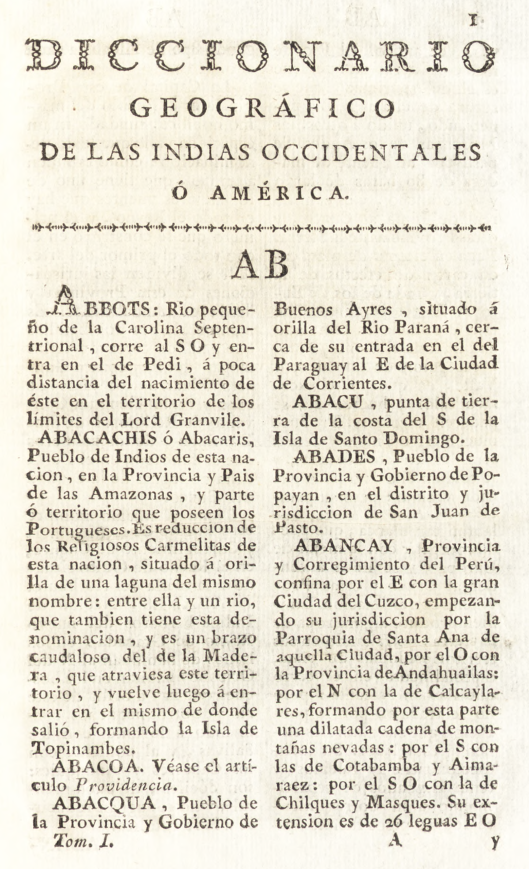
\includegraphics[width=\textwidth]{Dictionnaire1.png}
    \caption{Structure du Dictionnaire - Tome I.}
    \label{premFig}
\end{figure}


De plus, le Dictionnaire est une source très riche historiquement, géographiquement, et en matière de recensement. Dans les cinq tomes, il est possible d’y rencontrer tout ce qui concerne la constitution d’un lieu, comme la densité populationnelle, toute une série chronologique des découvertes, des conquérants, des fondateurs, des établissements religieux, comme les cathédrales et les évêques, de même que les événements naturels comme les incendies, les tremblements de terre et les invasions.

Toutes ces informations n’étaient pas sujettes à un traitement ou à une analyse spéciale dans le cadre de stage. Cependant, ce sont des informations très importantes, qui peuvent aider à la désambiguïsation des lieux. Car chaque lieu a une histoire et une caractéristique propre.



\clearpage
\section{Structuration des données}
\subsection{Structuration en XML : Le Projet HGIS de las Indias}

En partant du fichier que nous avons pu récupérer en collaboration avec le projet HGIS de las Indias\footnote{https://www.hgis-indias.net/}, son contenu était le texte brut du Dictionnaire et quelques poses de balises. Pour avoir eu ce texte brut à partir des images du Dictionnaire, il était nécessaire de passer par la technique de \Gls{OCR} qui permet la transformation d’une image en texte facilement utilisable. C’est une méthode généralement assez précise pour obtenir un texte clair, mais qui induit tout de même quelques erreurs dans la transcription de l’image en texte. 

Un premier balisage du texte avait été pensé par Werner Stangl dans le cadre de son projet \textit{HGIS de las Indias}. Pour délimiter les parties du Dictionnaire en paragraphes, il a choisi d’utiliser une balise div, avec un attribut « xml: id » en ordre chronologique des passages du Dictionnaire.\\
	

\begin{figure}[!h]
    \centering
    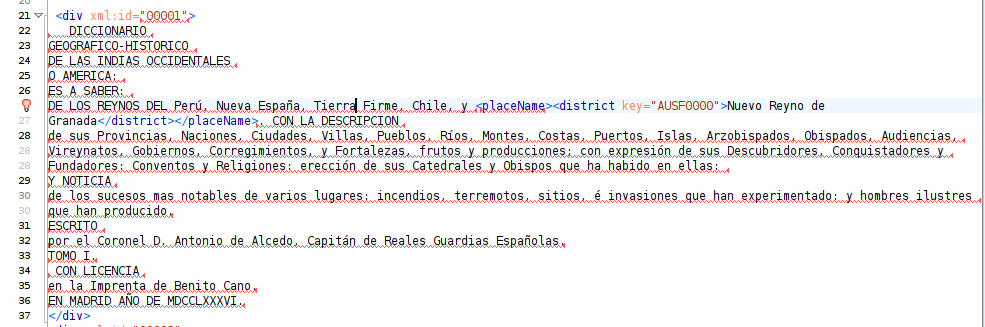
\includegraphics[width=15cm]{image2.png}
    \caption{Fichier initial avec des métadonnées - Tome I.}
    \label{deuxFig}
\end{figure}


Ce fichier a été associé directement au gazetier du Système d’information Géographique Historique de l’Amérique Hispanique (HGIS de las Indias), des années 1701-1808. La deuxième identification faite fut celle des lieux présentés dans le Dictionnaire d’Antonio de Alcedo. Ces derniers ont pu être identifiés par correspondance avec les localisations géographiques actuelles que l’on retrouve dans des bases de données telles que GeoNames. Pour les lieux identifiés, la balise div gagne un attribut settlement.\\
	
\begin{figure}[!h]
    \centering
    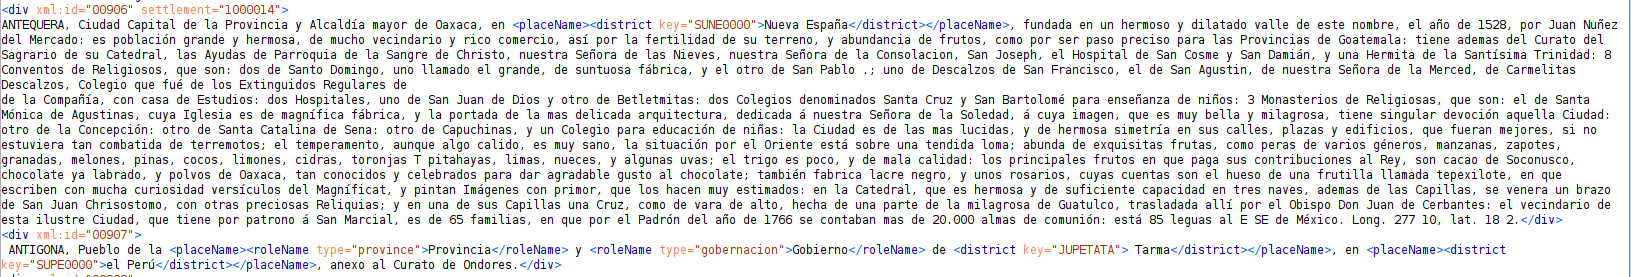
\includegraphics[width=18cm]{image3.png}
    \caption{Fichier initial avec des métadonnées: Le choix des balises - Tome I.}
    \label{troisFig}
\end{figure}	
	
	
La balise div se composent de trois descendants :\\

\begin{itemize}
    \item placeName : Nom de lieu.\\
    \item roleName : La description administrative qui a un attribut obligatoire, soit provincia, alcadia mayor où gobiernacion.\\
    \item district : La description géographique qui a aussi un attribut obligatoire key est une identification unique d’un lieu associé au gazetier du \Gls{HGIS de las Indias}.\\

\end{itemize}

Les attributs en div :\\
\begin{itemize}
   \item xml:id : numéro séquentiel des entrées.\\
    \item settlement : numéro référent aux lieux ayant une géolocalisation actuelle.\\
    \item Indigenas : pour identifier une entrée au sujet d’une tribu.\\
\end{itemize}

Le fait d’avoir dû récupérer une première interprétation de ce balisage auprès d’un autre projet représentait un défi supplémentaire pour moi, car il s’agissait de comprendre ce qui avait été fait auparavant, d’analyser les choix de balises et la stratégie suivie. Il n’aurait pas été possible de travailler avec ce fichier sans comprendre comment ce dernier fonctionnait et quelle stratégie il suivait. 

A partir de cette identification de la structuration du choix des balises dans le Dictionnaire d’Antonio de Alcedo, nous avons suscité un défi de travailler avec quelque chose de pré-établi, car nous devrons nous adapter à ces choix des modules pour réussir à structurée ces données.
	
	
\section{Les enjeux du processus}

L’enjeu technique principal de mon stage était  de structurer de manière la plus automatique possible le contenu du Dictionnaire. D’où l’intérêt de travailler avec l’encodage partiel du Dictionnaire qui nous a été transmis. A partir d’une analyse du Dictionnaire et du fichier avec quelques balises qui nous a été transmis, nous avons cherché dans un premier temps à récupérer toutes les informations liées à chaque entrée du Dictionnaire référant aux noms de lieux, ainsi que les informations administratives et géographiques. 

Étant donné que notre projet \textit{ANR TopUrbi} n’en était qu’à son point de départ et que nous avions récupéré les deux premières parties du processus par le projet \textit{HGIS de las Indias}, nous avons dû adapter notre stratégie suivant les fichiers qui nous ont été transmis. 
	
Nous avons alors dû faire un choix entre deux options, la première était d’adapter le choix des modules en Python en fonction du document que nous avons reçu, la deuxième était d’adapter le fichier  en fonction des modules avec lesquels nous étions le plus à l’aise.
	
\section{Implémentation du script python}

\subsection{La TEI}

Afin de travailler à partir du fichier initial, la structure des balises était en arborescence, nous avons d’abord pensé à mettre en place un script en langage de programmation Python qui servirait à automatiser le travail. Étant donné la taille de notre source, cinq tomes du Dictionnaire à traiter, utiliser un langage de programmation tel que Python nous permet d’accomplir ce qui était proposé pour les cinq mois de stage, à savoir de constituer une base de données du Dictionnaire. De plus, ce langage est abordable à tous niveaux, depuis le débutant jusqu’à l’utilisateur expérimenté. Il peut nous fournir une synthèse des informations en utilisant seulement quelques lignes de code.

Nous avons décidé de faire quelques modifications légères dans le fichier initial pour pouvoir le traiter au mieux. Nous avons pensé à mettre quelques indications de la \Gls{TEI}  qui est un langage développé depuis 1987 et qui vise à devenir un langage commun pour partager et  mutualiser les textes encodés numériquement\footnote{BURNARD, Lou. La TEI et le XML In : Qu’est-ce que la Text Encoding Initiative ? [en ligne]. Marseille : OpenEdition Press, 2015 (généré le 27 juillet 2022). Disponible sur Internet : <http://books.openedition.org/oep/1298>. ISBN : 9782821855816. DOI : https://doi.org/10.4000/books.oep.1298.} pour pouvoir en particulier utiliser le module en lxml\footnote{https://lxml.de} en langage de programmation en Python, ce module permet de manipuler des données en XML, et pour afficher nos résultats, nous avons choisi une sortie de fichier en CSV qui  signifie Comma-Separated Values et désigne un fichier informatique de type tableur, auxquels les valeurs sont séparées par des virgules. Ce fichier est un format simple qui permet de stocker une grande quantité de données et qu’il est possible d’utiliser avec différents outils et bases de données, dans différents contextes, ainsi que d’être lu par des tableurs tels qu’Excel et LibreOffice.

\begin{figure}[!h]
    \centering
    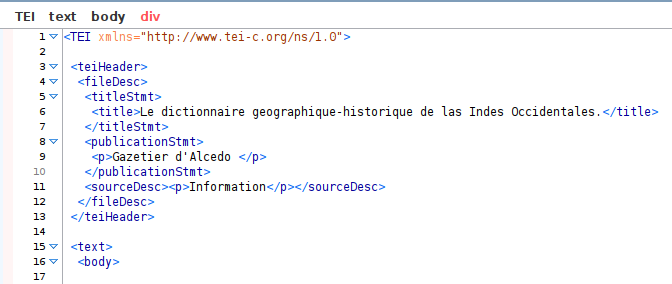
\includegraphics[width=15cm]{TEI.png}
    \caption{Adaptations en TEI du fichier initial - Tome I.}
    \label{quatFig}
\end{figure}


Cependant nous avons été confrontés à des difficultés pour l’extraction de l’information, car malgré quelques changements dans le fichier initial et les adaptations en XML TEI, le fichier n’était pas conforme aux recommandations de la TEI\footnote{https://tei-c.org/release/doc/tei-p5-doc/en/html/index.html}. De cette manière il pouvait être lu par le script comme un fichier \Gls{TEI}, mais le fichier contenait plusieurs problèmes tels que l’imbrication des balises, des balises ouvertes, les id qui commençaient par des chiffres alors que c’est interdit en TEI, ou encore le manque de spécifications de la ODD, ODT qui sont des spécifications de la personnalisation TEI pour le corpus.

De cette manière, nous n’avons pas pu demander à notre script de parcourir l’arborescence, à travers le module lxml, car les balisages n’étaient pas réguliers. Nous aurions par conséquent reçu des extraits d’informations différent à chaque fois, et nous aurions perdu beaucoup d’informations importantes. Nous avons donc opté pour partager le processus en deux, en utilisant les deux méthodes afin de parvenir à récupérer les informations des lieux de chaque entrée du Dictionnaire. \\

def detection\_descLieu(div):\\
  node = etree.strip\_tags(div,'*')\\
  return div.text\\

Avec le module lxml nous avons pu rentrer dans la balise principale div ; et dans div nous avons choisi d’utiliser le module re, en expressions régulières (regex) pour attraper les informations du reste des balises contenant les informations comme placeName, roleName et district. Les expressions régulières (regex), sont des expressions qui servent à faire des recherches dans un texte et à parvenir dans un résultat précis, selon nos indications. 

Comme exemple, je vous montre une partie de notre code. En sachant que chaque nom de lieu dans le Dictionnaire commence par les lettres capitales, nous avons pu demander dans notre fonction de matcher au travers d’une regex ces noms de lieux. Donc nous avons pu indiquer d’attraper tout en majuscules de A à Z, y compris les lettres de l’alphabet espagnol comme la lettre Ñ, en une ou plusieurs occurrences.\\

def detection\_nomLieu(line):\\
match = re.search(r' ([A-Z|Ñ|-]*)', line, re.DOTALL|re.MULTILINE)\\
if match:\\
return match.group(1)\\


L’application de cette regex a fonctionné car les entrées du Dictionnaire sont répétitives dans une même structure qui est propre aux noms de lieux. Nous avons dû faire une deuxième variation des regex pour repérer les noms des lieux, car il existe encore des noms composés auxquels nous avons dû faire une spécification plus complète, comme vous le verrez dans l’annexe. De cette manière nous avons pu trier les informations qu’on voulait récupérer dans des colonnes de notre tableur csv. 


\section{La base de données du Dictionnaire}

En utilisant la méthode décrite précédemment, nous avons pu créer un fichier sous la forme d’un tableau \Gls{CSV} dans lequel chaque colonne représentait l’information qu’on voulait récupérer du fichier initial. Notre idée principale était de conserver toutes les informations de chaque entrée du dictionnaire en relation avec des lieux. 

A la fin de chaque tome, il y a une liste de corrections et d’ajouts avec chaque nom de lieu, en gardant la même structure, le nom de lieux en premier en lettres capitales. Voir l'image \ref{cinqFig}. Ainsi, quand nous avons dû demander à notre script d’attraper toutes les lettres capitales de chaque entrée, nous avons pu récupérer ainsi des noms de lieux en double, pour ceux qui avaient des ajouts ou des corrections. Donc, dans un premier temps nous avons dû retirer cette liste des ajouts et des corrections, pour avoir seulement un lieu unique. Cependant de cette manière nous avons perdu des informations importantes pour la désambiguïsation, donc il sera nécessaire plus tard, quand cette étape de désambiguïsation sera plus avancée, de penser à une solution pour l’actualisation de ces informations.

\begin{figure}[!h]
    \centering
    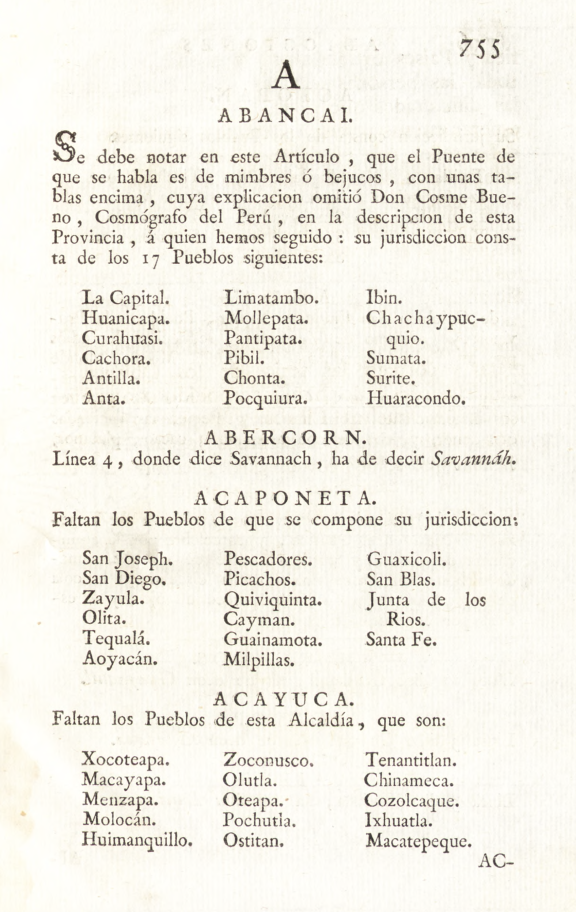
\includegraphics[width=\textwidth]{Dictionnaire2.png}
    \caption{Ajouts et corrections du Dictionnaire - Tome I.}
    \label{cinqFig}
\end{figure}

Nous avons choisi une première colonne id lieu qui fait référence à la chronologie des passages du Dictionnaire, en suite une deuxième colonne nom lieu reprenant les noms de lieux en majuscule, à la fois les noms simples ou composés. Ensuite, une troisième colonne settlement qui est un identifiant des lieux du gazetier HGIS de las Indias qui ont pu matcher avec d’autres bases de données géographiques. Si le résultat dans cette colonne est vide, c’est que les lieux trouvés n’avaient pas de correspondance dans le gazetier HGIS de las Indias. Pour finir, une dernière colonne type lieu fournit une description administrative particulière que de Alcedo avait choisi de faire (provincia, gobierno, etc.), desc lieu qui conserve toutes les informations de chaque entrée.

Au départ nous avions choisi de traiter uniquement les lieux qui n’avaient pas de correspondance avec la base de données de HGIS de las Indas, c’est-à-dire tous les lieux qui n’avaient pas reçu de numéro d’identification settlement. Bien que ceci fût le point de départ, nous avons souhaité constituer une base de données complète du Dictionnaire d’Antonio de Alcedo. Nous avons donc récupéré tous les lieux, y compris ceux avec un numéro d’identification dans la colonne settlement, et les autres lieux, ayant une identification settlement vide « NaN ».

Nous avons imaginé au début conserver la même méthodologie qui avait été utilisée pour les fichiers en XML, c’est-à-dire un fichier différent pour chaque tome. De cette manière nous avons obtenu un fichier csv différent pour chaque tome. Cependant par la suite nous avons revu ce processus pour n’appliquer le script qu’une seule fois au lieu de cinq, cela était plus pratique pour réussir à faire matcher les noms des lieux avec d’autres bases de données. 



\section{Pandas}

La deuxième partie de notre projet consistait à retrouver les coordonnées géographiques actuelles des lieux qui étaient décrits dans le Dictionnaire. Pour ce faire, nous avons eu besoin de faire des recherches au sein de plusieurs bases de données géographiques existantes.

Nous avons bien évidemment choisi de commencer nos recherches par la base de données HGIS de las Indias, ce qui permettait d’avoir la certitude que le fichier initial en XML était à jour par rapport à la base de données et que nous n’avions pas perdu d’informations dans la transcription. De plus la base de données HGIS de las Indias permettait d’élargir le périmètre puisqu’elle n’utilise pas que le Dictionnaire comme source, mais également d’autres sources se  rapportant à l’Amérique Hispanique du XVIIIe siècle.  

Pour commencer à traiter notre fichier csv, nous avons importé le module csv et pandas. J’ai choisi utiliser le module pandas\footnote{https://pandas.pydata.org/docs/user\_guide/index.html\#user-guide}, car c’est un langage simple, facile à utiliser et permettant de travailler avec deux fichiers en même temps : le fichier csv ainsi que le fichier xlsx du projet \textit{HGIS de las Indias}. Avec pandas, il est possible d’utiliser le DataFrame qui permet de structurer des données tabulaires en lignes et colonnes qui correspondaient aux deux types de fichiers que nous avions besoin de faire coïncider.

La première partie de notre script consistait à sélectionner les colonnes et les lignes dont nous avions besoin. L’objectif initial était en effet de traiter uniquement les lieux ayant une valeur nulle dans leur colonne settlement. Ensuite, il s’agissait de filtrer par la colonne type lieu tous les lieux correspondant à  « Pueblo, Nación,  Provincia, Isla, Ciudad,  Alcaldía », ce filtre était nécessaire car de Alcedo décrit également des noms de plantes, de tribus autochtones, etc. Et travailler avec ceci ne correspondait pas à l’objectif initial de ce stage. 

Nous avons créé une nouvelle colonne placeName pour laquelle nous avons sélectionné tous les nom lieu que nous avons transformés en minuscules grâce à la fonction \textit{lower()}. Il était important d’avoir les noms en écriture minuscule en effet car sans cela il aurait pu y avoir des problèmes de match si la machine cherchait à comparer un A majuscule avec un a minuscule par exemple, étant donné que tous les noms de lieux sont en minuscules dans la base de données HGIS de las Indias. Avant de pouvoir fusionner nos deux tableaux obtenus, nous avons utilisé la fonction \textit{drop()} qui permettait d’exclure la colonne settlement, qui n’était plus utile une fois que nous avions utilisé le filtre sur les noms de lieux. Pour finir, nous avons utilisé la fonction \textit{concat()} pour fusionner tous les tomes du Dictionnaire dans un seul et même fichier. Nous avons ainsi pu obtenir un seul fichier contenant toutes les informations importantes pour la suite, ce qui améliora beaucoup la visualisation des données. \\

Voici les premiers résultats de notre script :\\

 Tome I\\
\begin{itemize}
    \item entrées du dictionnaire : 5188
    \item noms de lieux par entrée avec le filtre sur type lieu : 1848\\

Tome II:\\
    \item entrées du dictionnaire : 3839
    \item noms de lieux par entrée avec le filtre sur type lieu : 1164\\

Tome III\\
    \item entrées du dictionnaire : 2427
    \item noms de lieux par entrée avec le filtre sur type lieu : 808\\

Tome IV\\
    \item entrées du dictionnaire : 3515
    \item noms de lieux par entrée avec le filtre sur type lieu : 1186\\

Tome V\\
    \item entrées du dictionnaire : 2849
    \item noms de lieux par entrée avec le filtre sur type lieu : 1248\\
\end{itemize}
Ainsi au total pour les cinq tomes, nous avons obtenu 6252 noms de lieux décrits dans le Dictionnaire d’Antonio de Alcedo qui correspondaient au filtre sur type lieu que nous avions appliqué, les autres entrées qui ne correspondaient pas à notre recherche étaient les parties introductoires du Dictionnaire, les listes, les corrections ou alors, la partie sur la flore et les peuples autochtones et etc.

Une fois filtrées les données du Dictionnaire, nous avons dû mettre en place quelques modifications dans la base de données HGIS de las Indias pour pouvoir commencer à matcher. Nous avons dû pour la deuxième partie de notre script mettre la base de données HGIS de las Indias au format Dataframe, afin que le module pandas puisse le lire et y faire des modifications. Nous avons ici aussi dû utiliser la fonction \textit{lower()} pour mettre tous les noms de lieux en minuscules, pour pouvoir faire le match avec notre base de données transformée auparavant. Ensuite toujours de la même façon, nous avons utilisé la fonction \textit{drop()} pour effacer les colonnes non utiles pour cet objectif. L’intérêt était en effet d’alléger la version du fichier pour le rendre moins long et moins lourd, et non pas de tout conserver, ce qui aurait induit un traitement beaucoup plus lourd et plus chronophage.

La troisième partie de notre script consistait à établir le lien entre les deux DataFrames. Nous avons pour cela utilisé la fonction \textit{merge()}. Afin de délimiter les conditions avec lesquelles nous voulions effectuer cette jointure, nous avons utilisé des paramètres \textit{on}, servant à indiquer dans quelles colonnes ou index nous voulions faire le point de jointure entre les deux tableaux. Nous avons choisi de faire la jointure dans la colonne placeName.

Nous avons de plus utilisé un deuxième paramètre, \textit{how}, qui permet d’indiquer par quelle manière nous allions faire la jointure entre les deux tableaux : par la gauche, par la droite, par l’intérieur, ou par l’extérieur. Nous avons ici eu recours à la jointure inner join, car c’est un type de jointure permettant de relier plusieurs tables entre elles.

Notre script a fonctionné et il a réussi à lire et à faire une jointure entre les deux tables. De  6252 noms de lieux recherchés du Dictionnaire dans la base de données Hgis de las Indias, nous avons eu un match de 1710 correspondances. Il nous restait à vérifier si le résultat de la jointure était satisfaisant. Pour une meilleure analyse de notre jointure et des résultats, nous avons choisi d’utiliser l’application Dataiku qui est une plateforme de Data Science collaborative, et qui permet le traitement analytique des données. La plateforme permet de préparer, mélanger, et modéliser, d’automatiser le workflow, et de déployer la production.

Notre premier objectif était d’avoir une vision générale de nos résultats, c’est-à-dire d’analyser si notre jointure avait été faite de la bonne manière, de pouvoir compter combien de types nous avions obtenus, de connaître un estimatif par région ou par pays et enfin de savoir à quoi correspondait nos résultats. En comparant les deux tables et si l’on regarde la description administrative des lieux, nous nous sommes d’abord rendu compte qu’il existe beaucoup plus de types dans la base de données HGIS de las Indias qu’il y en a dans le Dictionnaire d’Alcedo. \\

	Le Dictionnaire d’Alcedo, se caractérise comme suit :\\
	
\begin{itemize}
\item Pueblo : 1753
\item Provincia : 7
\item Isla : 3
\item Nación : 3
\item Ciudad : 1\\
\end{itemize}

Dans le gazetier HGIS de las Indias :\\

\begin{itemize}
\item Pueblo : 643
\item Localidad : 383
\item Rural : 325
\item Poblacion: 286
\item Fuerte : 83
\item Villa: 23
\item Parcialidad : 16
\item Ciudad : 8\\
\end{itemize}
Par rapport aux régions en correspondance avec les pays actuels, nous avons pu constater :\\
\begin{itemize}
\item PERU : 349
\item ARG : 206
\item MEX : 205
\item COL : 169
\item BOL : 118
\item CUB : 108
\item PAN : 61
\item URY : 60
\item CHL : 56\\
\end{itemize}

Savoir ces informations est très important pour les choix des bases de données géographiques que nous pourrons dans l’avenir saisir pour rencontrer des informations sur une région déterminée. Il faut avoir en tête que la base de données HGIS de las Indias, utilise plusieurs sources et non seulement le Dictionnaire de Alcedo, donc c’est pour ça qu’il y a plusieurs types de lieux, qu’on ne rencontre pas chez de Alcedo.

Le premier constat fut de se rendre compte qu’effectuer une jointure simple en reliant simplement les noms de lieux tout en se fiant à leur orthographe allait occasionner plusieurs doutes quant à la véracité des informations. Le problème principal était effectivement l’orthographe. Antonio de Alcedo utilise une orthographe propre à lui dans son Dictionnaire, qui dépendait de comment il comprenait le nom de l’endroit, ou comment il l’entendait à l’oral ; de l’autre côté Werner Stangl utilise l’orthographe de plusieurs sources différentes pour constituer son gazetier HGIS de las Indias. Ici aussi un auteur pouvait écrire un nom de lieu d’une manière totalement différente selon sa propre compréhension. Ainsi de cette manière faire une jointure allait occasionner de nombreuses erreurs, par exemple en reliant deux lieux du même nom mais situés dans des régions différentes, d’autres groupes de mots ayant aussi changé d’orthographe, par exemple des noms de lieux qui étaient écrits GU avaient évolués vers HU, ou encore X en J, ou GI en JI ou encore GE en JE, etc.    	

Nous avons fait une jointure en reliant la colonne placeName que nous avons pu créer, et la colonne nombre du gazetier HGIS de las Indias. Cependant, il aurait mieux valu, pour commencer, de faire une jointure entre la colonne placeName et la colonne label. Car en faisant un match avec la colonne nombre de la base de données Hgis de las Indias, est le nombre actuel du lieu, après les changements dans le temps et la colonne label est le nom autant que dans les sources du XVIIIe siècle, donc nous aurions peut-être plus de chance d’avoir une correspondance.

Pour l’avenir du projet il sera nécessaire de penser à ces problématiques, comment relever le défi de la désambiguïsation des lieux et avoir une stratégie pour la véracité des données. Je parlerai un peu plus de la désambiguïsation des lieux dans le chapitre quatre, cependant en étant encore dans les bases de données géographiques, nous avions commencé à faire un test avec une deuxième base de données, GeoNames, et je vous présenterai un peu ce que nous en avons pensé et également ce qui sera nécessaire pour la conclusion cette étape inachevée.

\section{GeoNames}

GeoNames est une base de données géographiques gratuite et en open accès, cette base comporte 25 millions de noms géographiques, soit plus de 11 millions de lieux avec leurs coordonnées géographiques (dont 4,8 millions de lieux habités) et 13 millions de lieux autres, non géoréférencés. Nous avons mis en place une stratégie visant à pouvoir localiser les données géographiques des noms de lieux décrits dans le Dictionnaire d’Alcedo en utilisant la base GeoNames\footnote{http://www.geonames.org/}. 

Le processus est presque similaire au processus décrit en utilisant la base de données Hgis de las Indias, il change seulement par quelques modules utilisés que je vais vous expliquer. Pour ce faire, nous avons préparé un script en Python qui permettrait de faire matcher les deux bases de manière automatique. Nous avons dû installer la librairie geocoder, qui est une librairie nécessaire lorsque des coordonnées géographiques sont traitées. Nous avons ensuite importé les trois packages nécessaires afin de travailler dans les bonnes conditions avec notre base de données du Dictionnaire et de la base GeoNames, c’est à dire csv, pandas, et geocoder.

Pour la première partie du script, nous nous sommes intéressés à notre ficher en csv, sur lequel nous avons sélectionnés à nouveau uniquement les colonnes utiles, c’est-à-dire celles avec les settlement de valeur nulle. Parmi les données restantes, nous avons utilisé un filtre par type lieu pour ne conserver que les types « Pueblo, Nación,  Provincia, Isla, Ciudad,  Alcaldía ». Ensuite, nous avons pu passer à l’étape suivante qui consistait à récupérer les informations et d’essayer de les faire correspondre avec celles de la base de données GeoNames, au travers d’une \Gls{API}\footnote{https://realpython.com/api-integration-in-python/} qui est un programme qui permet à deux applications distinctes de communiquer entre elles et d’échanger leurs données. Donc, à partir de cet API il serait possible de faire communiquer la base de données du Dictionnaire avec la base de données Geonames.

Si le résultat obtenu s’avère être positif, le script nous retourne alors un OK et indique entre crochets le nom correspondant au nom de lieux qu’on recherche. Voir l'image \ref{sixFig}. Ce type de match est très intelligent et précis, car même si le nom n’est pas écrit de la même manière entre les lieux du Dictionnaire et la correspondance dans GeoNames, l’outil peut afficher comme une correspondance positive. D’un autre côté, si le script ne retrouve aucune correspondance dans la base GeoNames, il affiche une erreur.\\
	

\begin{figure}[!h]
    \centering
    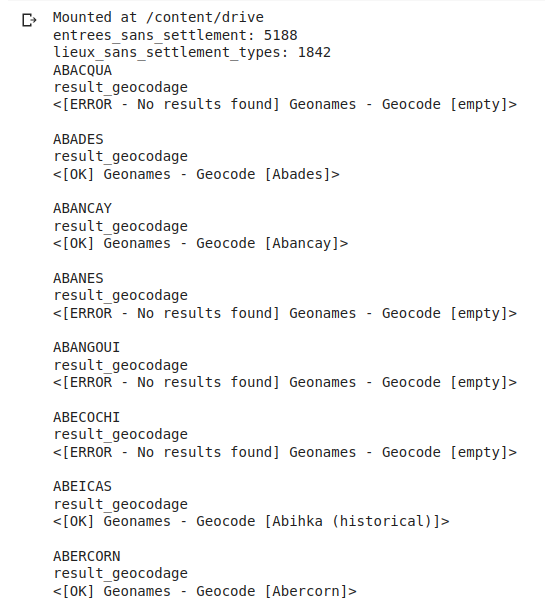
\includegraphics[width=15cm]{image04.png}
    \caption{Résultat de la recherche des lieux}
    \label{sixFig}
\end{figure}

Une problématique rencontrée ici est que le processus peut renvoyer parfois des faux positifs ou encore des faux négatifs, compliquant l’analyse. L’orthographe est encore une fois une première source d’erreur, et sélectionner un seul critère pour ce type de match est une opération risquée. Cependant à ce stade du stage, nous n’avons pas poursuivi davantage d’investigations. Nous nous sommes simplement intéressés à comprendre la meilleure manière de préparer le script, et les besoins primordiaux pour établir les bons matchs entre les deux bases de données. Pour l’avenir du projet, cela sera une étape cruciale, il faudra réfléchir à comment lever les ambiguïtés qui peuvent exister. 

De mon point de vue, il s’agirait d’abord de se concentrer à terminer la correspondance entre les lieux décrits dans le Dictionnaire et ceux de la base de données HGIS de las Indias et affiner les matchs reçus pour enlever toutes les ambiguïtés. En effet Werner Stangl s’est lui-même inspiré de la base de données GeoNames pour construire sa base de données HGIS de las Indias. Une fois cela réalisé, nous pourrions affiner l’étude en lançant une deuxième recherche utilisant uniquement les noms de lieux non retrouvés dans la base de données HGIS de las Indias et de relancer un script pour rechercher des correspondances avec GeoNames. 

Ce processus de construction d’un processus automatique et de l’analyse des résultats était une étape très riche  en apprentissage lors de mon stage, car j’ai pu essayer de comprendre les résultats et de chercher des solutions aux problèmes, ainsi qu’à être en communication avec l’équipe du projet, des gens plus expérimentés comme Carmen Brando dans la feuille des textes et dans les langages de programmation, ainsi que Werner Stangl pour les connaissances acquises lors de son projet Hgis de las Indias et également sur l’Amérique Hispanique du XVIIIe siècle.

Comme nous avons pu voir comment faire pour avoir les bons résultats, au long de ce processus d’automatisation des tâches et de réflexion. Nous avons pu voir ce qui serait essentiel pour le projet, rencontrer une manière de faire la désambiguïsation des lieux et que malgré notre script en python était capable de faire des recherches sur les bases de données cependant nos filtres, nous avons dû réfléchir à une deuxième possibilité de parvenir à notre objectif, donc nous avons pensé au Traitement automatique des langues et je vous présenterai comment nous avons envisagé cela dans le prochain chapitre.  

\part{Traitement automatique des langues}
	
	\chapter{}
	\section{Traitements pour une annotation manuelle du Dictionnaire Alcedo en vue d’une segmentation automatique et sémantique de son contenu.}
	
Comme vous l’avez vu auparavant, nos méthodes initiales de match n’étaient pas tout à fait satisfaisantes lors des problèmes rencontrés, au sujet de l’orthographe par exemple. Nous avons dû réfléchir à l’une des possibilités de régler ces problèmes de désambiguïsation des lieux, qui consistait à utiliser une application permettant de faire du \Gls{TAL} pour la reconnaissance des entités nommées.

Le Traitement automatique des langues TAL est une discipline interdisciplinaire faisant un lien entre la linguistique et l’informatique. Son objectif est de développer des applications ou des programmes informatiques capables de traiter automatiquement des données linguistiques tout en prenant en compte les spécificités du langage humain. À l’aide de ces outils, l’enjeu consiste à la base que, pour comprendre un document, il faut reconnaître les informations pertinentes dont on parle et qui jouent un rôle dans la description d’un événement, d’un fait. L’objectif des entités nommées est de repérer ces éléments. Le processus consiste en premier lieu à reconnaître les identités nommées du document, à définir les frontières et leur catégorisation. La notion d’entités nommées, ce pourrait être des noms propres, des noms de lieux, des organisations, des expressions numériques, comme les dates, une monnaie etc\footnote{Nouvel, Damien, Maud Ehrmann, et Sophie Rosset. Les entités nommées pour le traitement automatique des langues. ISTE Group, 2015. https://books.google.fr/books?id=djVgDwAAQBAJ\&printsec=frontcover\&redir\_esc=y\#v=onepage\&q\&f=false.}.

Nous avons choisi l’application tagtog\footnote{https://www.tagtog.com/} qui est un outil d’annotation du texte permettant d’annoter et de normaliser les entités nommées. Il est par exemple possible d’ajouter des étiquettes d’entités, des relations, et même de faire plusieurs niveaux d’annotations. Il s’agit de plus d’une plateforme collaborative, permettant de travailler en équipe sur le même texte, et offrant la possibilité de voir toutes les modifications effectuées par un autre membre de l’équipe. Cette annotation manuelle a pour objectif de faciliter la désambiguïsation des lieux de notre base de données géographique du Dictionnaire d’Alcedo.
	
Dans le cadre du stage, Carmen Brando et moi-même voulions essayer cette plateforme et y définir quelques paramètres initiaux afin de savoir si l’application répondrait bien à nos exigences. Nous avons également souhaité voir notre comptabilité en relation à la compréhension de la définition des entités nommées; et enfin faire quelques tests qui permettraient de nous rendre compte des problématiques que nous allions rencontrer lors du traitement et pouvoir en discuter avec les spécialistes de l’histoire de l’Amérique Hispanique du XVIIIe siècle du projet \textit{ANR Top Urbi}.

Avec l’application tagtog il est possible de créer un modèle général que l’on peut ensuite appliquer à tout notre corpus. Pour créer ce modèle, il est nécessaire d’écrire des annotations sur un pourcentage significatif de notre Dictionnaire. Une fois les annotations faites, il faudra vérifier que le modèle parvient bien à reconnaître les entités nommées sur la base de nos annotations. Si le résultat est positif, nous devrions par la suite pouvoir appliquer le modèle de manière automatique à tout le reste du corpus non annoté. 

La première étape a donc été de récupérer un pourcentage significatif de notre Dictionnaire afin que nous puissions travailler dessus. A l’aide d’un script Python, nous avons choisi de récupérer 5\% du nombre d’entrées de chaque tome, pour que nous puissions les annoter à la main au travers de l’application tagtog. Ceci aura été le point de départ pour la création de notre modèle. 

Pour le fonctionnement du script, il fut nécessaire d’utiliser des modules, csv, glob, pandas, requests et os. Le module glob par exemple recherche tous les chemins correspondant à un motif particulier. Nous l’avons utilisé, car il était nécessaire de demander que le script lise tous les fichiers en csv au même temps. Le module os fournit quant à lui des fonctions permettant d’interagir avec le système d’exploitation. Le module requests permet d’utiliser le protocole http. Ce module est nécessaire lorsque nous voulons récupérer des informations d’un site web au travers d’une \Gls{API}.
	
Une fois que la première partie du script a tourné, voici les nombres d’entrées par tome qui ont été envoyés à l’application tagtog et qui étaient prêts pour l’annotation.\\
	
	\textbf{Corpus et échantillon à annoter}\\

 \noindent \textbf{Tome I}
\begin{itemize}
\item Nombre d'entrées: 5276
\item Nombre d'entrées d'un échantillon aléatoire(5\%): 264 \\
\end{itemize}
\textbf{Tome II}
\begin{itemize}
\item Nombre d'entrées: 3902
\item Nombre d'entrées d'un échantillon aléatoire(5\%): 195\\
\end{itemize}
\textbf{Tome III}
\begin{itemize}
\item Nombre d'entrées: 2649
\item Nombre d'entrées d'un échantillon aléatoire(5\%): 132 \\
\end{itemize}
\textbf{Tome IV}
\begin{itemize}
\item Nombre d'entrées: 3571
\item Nombre d'entrées d'un échantillon aléatoire(5\%): 179 \\

\end{itemize}
\textbf{Tome V}
\begin{itemize}
\item Nombre d'entrées: 3566
\item Nombre d'entrées d'un échantillon aléatoire(5\%): 178 \\
\end{itemize}

Avant de commencer l’annotation des entités nommées, une étape très importante est celle de la compréhension de nos besoins sur la base de l’objectif du projet et notre compréhension du Dictionnaire. Nous avons besoin de définir les entités nommées que nous allons utiliser pour chacune des entrées\footnote{Nouvel, Damien, Maud Ehrmann, et Sophie Rosset. Les entités nommées pour le traitement automatique des langues. ISTE Group, 2015. p.14  https://books.google.fr/books?id=djVgDwAAQBAJ\&printsec=frontcover\&redir\_esc=y\#v=onepage\&q\&f=false.}.

Sur le principe nous avons pensé à deux possibilités d’annotation. La première possibilité serait une annotation au niveau des entrées permettant de les classifier en distinguant les entrées de lieux et les entrées correspondant à d’autres classes, par exemple la faune, la flore ou encore les homonymes. La deuxième possibilité est une annotation au niveau des mots dans une entrée pour permettre de repérer les noms de lieux, les catégories des lieux et les références spatiales de situation géographique.

A ce stade du projet, c’est précisément les noms propres des lieux qui nous intéressent, avec bien-sûr les expressions lexicales qui désignent la nature, la fonction ou encore le type d’un lieu. Ainsi nous avons choisi les catégories d’annotation suivantes en tagtog :\\

\noindent \textbf{Titre : d’une entrée}\\
\begin{itemize}
\item Tous les noms de lieux, simples ou composés. Tout ce qui est le sujet de l’entrée.
\item Tous les noms des rivières, lagunes, peuples indigènes.\\
 \end{itemize}   
\textbf{Type : type/nature/fonction d’un lieu (ou autre) décrit dans une entrée du dictionnaire}\\
\begin{itemize}

\item Type/nature/fonction d’une entrée simple ou composées.
\item Rivières, îles, mers.
\item Villes, provinces, gouvernements etc.\\
\end{itemize}   
\textbf{Lieu : nom de lieux dans le texte d’une entrée}\\ 
\begin{itemize}
\item Tous les lieux géographiques tels les noms des villes, des villages, des pays, des régions ou des royaumes.\\
\end{itemize}
\textbf{Démonyme}\\
\begin{itemize}
\item Tous les noms relatifs aux tribus indigènes, aux plantes, aux nominations des personnes, qu’ils soient en espagnol, français ou encore dans la langue locale.\\
\end{itemize}
\textbf{Personne}\\
\begin{itemize}
\item Quand il y a une personne dénommée ou quand un lieu est appelé par un nom de personne.\\
\end{itemize}
\textbf{Les annotations}\\

Les annotations sont distinguées par des étiquettes de couleurs différentes, comme vous allez le rencontrer dans les exemples ci-dessous dans ces spécifications.\\
\begin{itemize}
\item Vert: Titres
\item Violet: Types
\item Jeune: Lieux
\item Bleu: Démonymes
\item Rouge: Personnes\\
\end{itemize}

Après avoir effectué le choix des étiquettes, nous nous sommes lancées avec Carmen Brando à la mise en place manuelle des étiquettes. Voici plus bas quelques exemples annotés. La première problématique fut de bien choisir les étiquettes en fonction des informations que nous souhaitions récupérer. Cette partie est l’enjeu le plus important, car le choix stratégique n’est pas évident à faire.

Pour un premier essai, nous avons choisi d’utiliser quelques petites étiquettes, et nous avons essayé de définir cinq étiquettes sur les noms de lieux, le type, la localisation géographique, le démonyme et le nom de personnes. Avec l’outil tagtog nous avons choisi les vingt premières entrées pour pouvoir commencer l’annotation des entités nommées. L’objectif était de voir notre correspondance par rapport à la compréhension de la catégorisation de l’information. Nous avons reçu un taux de correspondances très bas.

Cependant, ce premier essai pilote nous a permis de comprendre de quoi nous avions besoin pour affiner encore plus le choix des étiquettes, étant donné qu’il y avait des cas très particuliers à traiter. En effet, nous avons annoté les vingt premières entrées du Dictionnaire, qui faisaient toutes partie du tome V, le tome qui parle de manière la plus approfondie de la nature, par exemple concernant les îles, les montagnes, etc. Nous nous sommes rendu compte qu’il était plus judicieux de choisir plutôt cinq entrées de chaque tome. Nous avons donc annoté vingt-cinq entrées au total qui permettaient d’avoir un aperçu des difficultés que nous pourrions rencontrer dans chaque tome, et ainsi obtenir des cas multiples. 
	
	
\begin{figure}[!h]
    \centering
    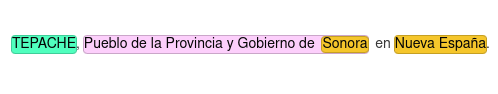
\includegraphics[width=15cm]{image5.png}
    \caption{Annotation des entités nommées - Tome V, id = 16020.}
    \label{septFig}
\end{figure}


Vous pouvez voir ci-dessus une entrée du dictionnaire de manière structurée. En vert nous avons fait ressortir le titre de l’entrée, c’est-à-dire le nom du lieu que nous cherchons à retrouver ; en violet le type et enfin en jaune la localisation du lieu. Dans ce cas, je me suis posé plusieurs questions, et j’ai rencontré plusieurs problématiques. Par exemple en rapport avec l’étiquette en violet représentant le type ou la fonction de ce lieu. Par manque de connaissance approfondie sur l’histoire administrative coloniale de l’Amérique Hispanique du XVIIIe siècle, je me suis posé la question de ce qui devait exactement être englobé en violet : toute la description ? Ou encore Pueblo de la Pronvincia y Gobierno comme je l’ai fait ? Ou enfin seulement pueblo, provincia y gobierno ?

\begin{figure}[!h]
    \centering
    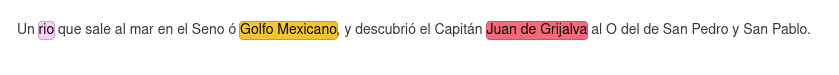
\includegraphics[width=15cm, height=2cm]{img1.png}
    \caption{Annotation des entités nommées - Tome V, id = 15487.}
    \label{huitFig}
\end{figure}
	
\begin{figure}[!h]
    \centering
    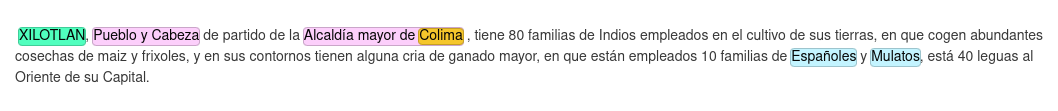
\includegraphics[width=15cm, height=2cm]{image06.png}
    \caption{Annotation des entités nommées - Tome V, id = 17774.}
    \label{neufFig}
\end{figure}

\begin{figure}[!h]
    \centering
    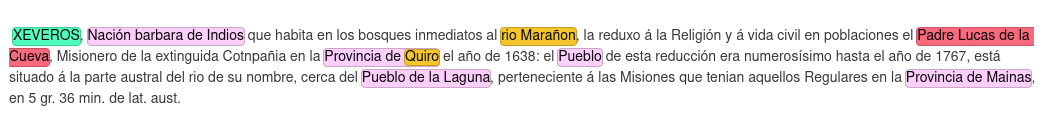
\includegraphics[width=15cm, height=2cm]{image07.png}
    \caption{Annotation des entités nommées - Tome V, id = 17750.}
    \label{dixFig}
\end{figure}

Après avoir fait avec Carmen Brando la pose des entités nommées en même temps, chacune avec son compte, sur la même quantité des entrées et sur les mêmes entrées, dans l’outil tagtog, il a été possible d’analyser des statistiques des correspondances entre les membres du projet sur les annotations faites dans la partie métrique. Les résultats ont été divisés en types d’annotations (types d'entités, d’étiquettes, d'entités, d’étiquettes de documents, normalisations et relations). Pour chaque tâche d'annotation, les scores ont été affichés sous forme de matrice. Chaque cellule représente la paire d'accord pour deux annotateurs, soit 100\% le niveau d'accord maximum et 0\% le minimum. Le pourcentage d'accord près du titre de chaque tâche, d'annotation, représente l'accord moyen pour cette tâche d'annotations\footnote{https://docs.tagtog.com/collaboration\#iaa-inter-annotator-agreement}.\\

\textbf{Pour les types entités, nous avons eu un score de correspondance :}
\\
\begin{itemize}
    \item Lieu :  38.64\%
    \item Personne : 100\%
    \item Titre : 5\%
    \item Type : 0\%
    \item Démonyme : 0\%\\
\end{itemize}
	
Si l’on analyse les entrées que nous avons pu annoter, la première problématique à penser est celle d’éventuels problèmes d'erreurs \Gls{OCR}, par exemple nous pouvons voir Quiro à la place de Quito. Il sera nécessaire d’annoter tout de même les variations des noms de lieux et les types, sinon lorsque nous appliquerons le modèle d’annotation automatique, il ne pourra pas reconnaître Quiro comme un nom de lieu par exemple.

Nous avons ensuite pu apercevoir que les catégories que nous avions choisies en premier lieu ne correspondaient pas tout à fait à la complexité des entrées du Dictionnaire, il aura donc été nécessaire de les modifier ou d’en ajouter des nouvelles. Des questions se sont posées alors de savoir si l’on devrait ajouter une étiquette pour définir des expressions temporelles, ou pour les coordonnées de localisation. Cela nous aiderait sûrement à donner plus de précisions sur la localisation géographique des lieux. Même raisonnement pour les pueblos indígenas, car à l’époque  co-existaient plusieurs peuplements indigènes dans les différentes parties des Amériques, ce qui n’est plus le cas aujourd’hui. Donc nous en sommes restées à la question de savoir si nous devions créer une nouvelle étiquette ou appliquer l’étiquette titre pour les noms de lieux référant aux peuplements autochtones. On devrait alors créer une étiquette pour les congrégations, par exemple les cappuccinos, jésuites, etc.

Par rapport aux démonymes, nous avons dû également faire la distinction entre les Européens et les autochtones ? Devions-nous également conserver ou non les étiquettes pour les noms de personnes ? Cela pourrait-il nous aider à la désambiguïsation des lieux ? Il faudrait également créer une étiquette pour les corps de métiers, par exemple los botanicos. Une possibilité serait par exemple de distinguer les types\_lieux de types\_autres, pour apprendre au modèle à les distinguer de manière automatique. Pour les types\_autres, nous privilégions les types désignés avec un vocabulaire courant, par exemple nous évitons les noms scientifiques des espèces de plantes. Pour les noms raccourcis de lieux, inclure la préposition “de” , par exemple “de Tabago”, dans la structure des entrées du Dictionnaire de Alcedo la nature du lieu n’est pas précisée de suite dans le contexte immédiat mais un peu plus loin.

Pour travailler sur toutes ces questions préliminaires, nous avons collaboré un moment avec Werner Stangl, qui a construit la base de données HGIS de las Indias et qui connaît très bien le Dictionnaire de Alcedo. Il nous a donc aidées de ses connaissances sur le sujet afin d’arriver à trouver quelques réponses. Werner Stangl nous a suggéré de créer les étiquettes suivantes : \\
	
	\begin{itemize}
    \item Division\_1 : royaume, audience.
    \item Division\_2 : les districts (Provincia, jurisdicción, alcaldía mayor, gobierno et etc.)
    \item Settlement : nom de lieu dans le texte d’une entrée
    \item Landmark : un bâtiment ou un lieu facilement reconnaissable
    \item Démonyms : noms de peuples
    \item Persons :  noms de personnes	\\
\end{itemize}	

L’apport de Werner Stangle sur les annotations est intéressant : noter la division des lieux du point de vue hiérarchique entre les divisions 1 et 2, créer une étiquette settlement, ce qui garde un lien avec le fichier des balisages initial, que nous avons pu voir dans le chapitre trois et avec notre base de données du Dictionnaire de Alcedo. Ce premier essai nous a apporté énormément sur la connaissance de notre source sur laquelle nous travaillons, le fait de faire des annotations des entités nommées et de mesurer nos compatibilités entre les membres de l’équipe, a enrichi nos connaissances, nous a permis le partage d’informations et nous a fait comprendre les enjeux de ce type de stratégie pour le projet \textit{ANR Top Urbi}. Le traitement automatique des langues a été une première expérience très enrichissante pour moi, d’apprendre à travailler avec le souci du détail et en collaboration avec une équipe. Cela nous a fourni un point de départ et une première réflexion sur le sujet. Cependant, l’idée a besoin de mûrir davantage et d’être discutée avec l’ensemble du comité scientifique auprès des historiens, anthropologues, géographes, archéologues, sociologues, linguistes, etc. ce qui est déjà prévu pour la suite du projet.

\section{Cartographie moderne des Indes Occidentales}

La dernière étape du projet numérique consiste à établir une cartographie moderne des Indes Occidentales en partant de la base de données géographiques du Dictionnaire historique et géographique des Indes Occidentales d’Antonio de Alcedo (1786-1789). Dans le cadre du projet \textit{ANR Top Urbi}, l’équipe compte utiliser le logiciel QGIS qui est un logiciel de Système d’Information Géographique (SIG) en open source, développé par un projet officiel de la fondation \Gls{OSGeo}.

Le point de départ d’une transcription d’une cartographie vers le SIG est bien sûr un support traditionnel pour l’information géographique : les cartes et les fiches manuelles. Puisque toutes les cartes comportent des composantes géométriques et topologiques, il est possible depuis les années 1980 de transcrire l’information physique (sur papier) en information numérique. Les processus de transcription numérique passent d’abord par un enregistrement des fiches et manuscrits sous forme de tableurs ou bases de données, et de les passer par un système de gestion de la base de données ou SGDB, qui est un logiciel permettant de stocker, récupérer, ajouter, supprimer ou encore modifier des données. Il est également possible de numériser des cartes et plans vers le logiciel DAO, qui est un outil de dessin assisté par ordinateur permettant de produire des dessins techniques via un logiciel informatique. 

Une fois les données numériques créées, l’étape suivante consiste à intégrer ces informations numériques, soit \Gls{SGBD} ou \Gls{DAO}, afin de créer des Systèmes d’information géographique (SIG). Enfin la dernière étape sera de passer du logiciel de bureau vers des services web, à travers l’utilisation de portails géographiques. 

Pour effectuer un bon traitement des informations dans un Système d’Information Géographique, il existe six points essentiels sur lesquels il faut se pencher. Il faut d’abord pouvoir faire abstraction du monde réel, car le SIG est une représentation. Il est nécessaire d’acquérir les données pour la saisie d’informations géographiques sous forme numérique. Gestion de base de données, mises en forme et visualisations des données, manipulations et interrogations des données géographiques.

Une carte géolocalisée est un fichier informatique représentant une image d’une portion de la surface terrestre munie des coordonnées géographiques précises. Avec le système de cartes anciennes l’idée est d’ouvrir une image dans un système d’informations géographiques où l’image est disposée dans un système de coordonnées de référence, de manière à ce que les deux images qui correspondent à la même zone soient superposées\footnote{Audelan, Claire, Marion Humbert, Clémence Lescuyer, Constance de Vergnette de la Motte, et sous la direction d’Alain Guerreau. « Géolocaliser des cartes anciennes : procédure ». Bulletin du centre d’études médiévales d’Auxerre | BUCEMA, no Hors-série n° 9 (29 février 2016). p.2.  https://doi.org/10.4000/cem.14148.}. 

Dans un premier temps, nous avons essayé de fournir une représentation cartographique moderne de la carte de Francisco Requena datée de 1796. Nous avons choisi cette carte, car elle est l’une des sources cartographiques importantes pour étudier la délimitation des territoires en Amérique du Sud. Francisco Requena travaillait pour la Couronne Espagnole au XVIIIe siècle en tant qu’ingénieur en chef, et il dessina une carte qui avait pour objectif d’accompagner la réflexion sur le projet de démarcation des limites entre les territoires propres aux Couronnes Espagnole et Portugaise. 

La première question est de comment faire le géoréférencement d’une carte ancienne avec de la géolocalisation actuelle? Nous allons voir un exemple avec la carte de Francisco Requenha.\\


\begin{figure}[!h]
    \centering
    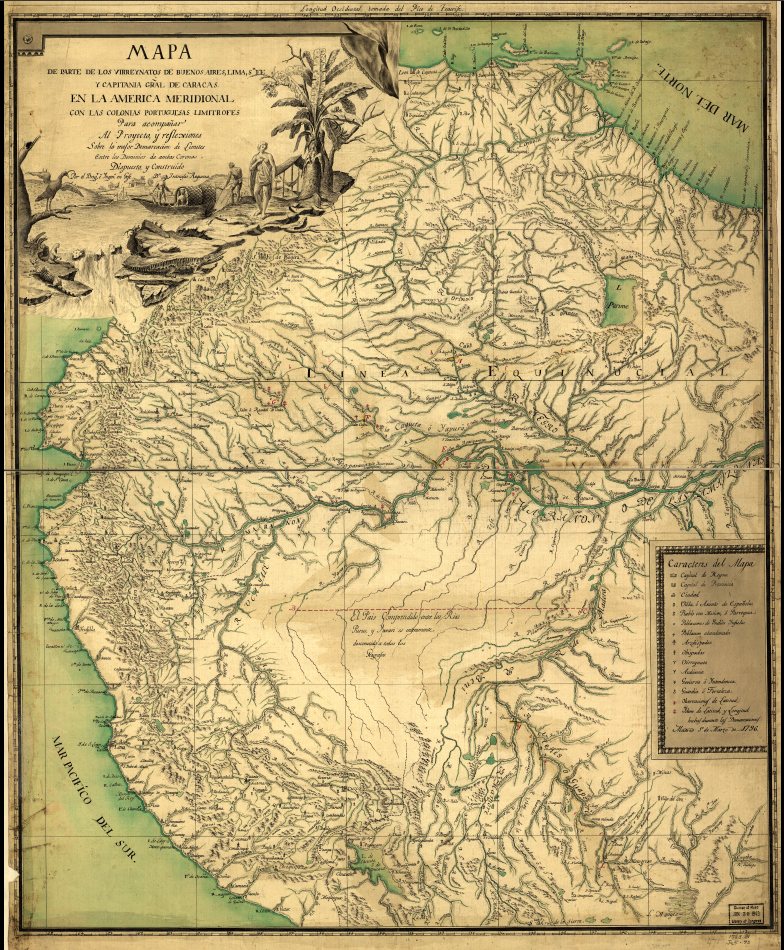
\includegraphics[width=15cm]{Requena carte.png}
    \caption{Carte de Francisco Requena(1796).}
    \label{onzeFig}
\end{figure}

Le processus de géolocalisation consiste à indiquer les coordonnées exactes par un nombre suffisant de points sur l’image qu’on traite. Donc nous avons dû identifier précisément ce que représente cette carte et l’espace qu’elle occupe dans l’Amérique du Sud. En travaillant avec les systèmes des couches et avec la transparence du logiciel Qgis, nous avons essayé dans un premier temps de repérer des endroits toujours concordants dans la carte ancienne et dans la carte actuelle, comme les noms des grandes villes, des fleurs, ou des bâtiments historiques. Cependant il n’est pas toujours évident de trouver des correspondances car les territoires évoluent au fur et à mesure des siècles. A partir de l’identification des lieux-clés, nous avons pu au travers de l’application des points de correspondances entre notre carte ancienne et notre carte actuelle établir une première correspondance entre nos deux cartes, comme vous pouvez le voir dans la deuxième image.

\begin{figure}[!h]
    \centering
    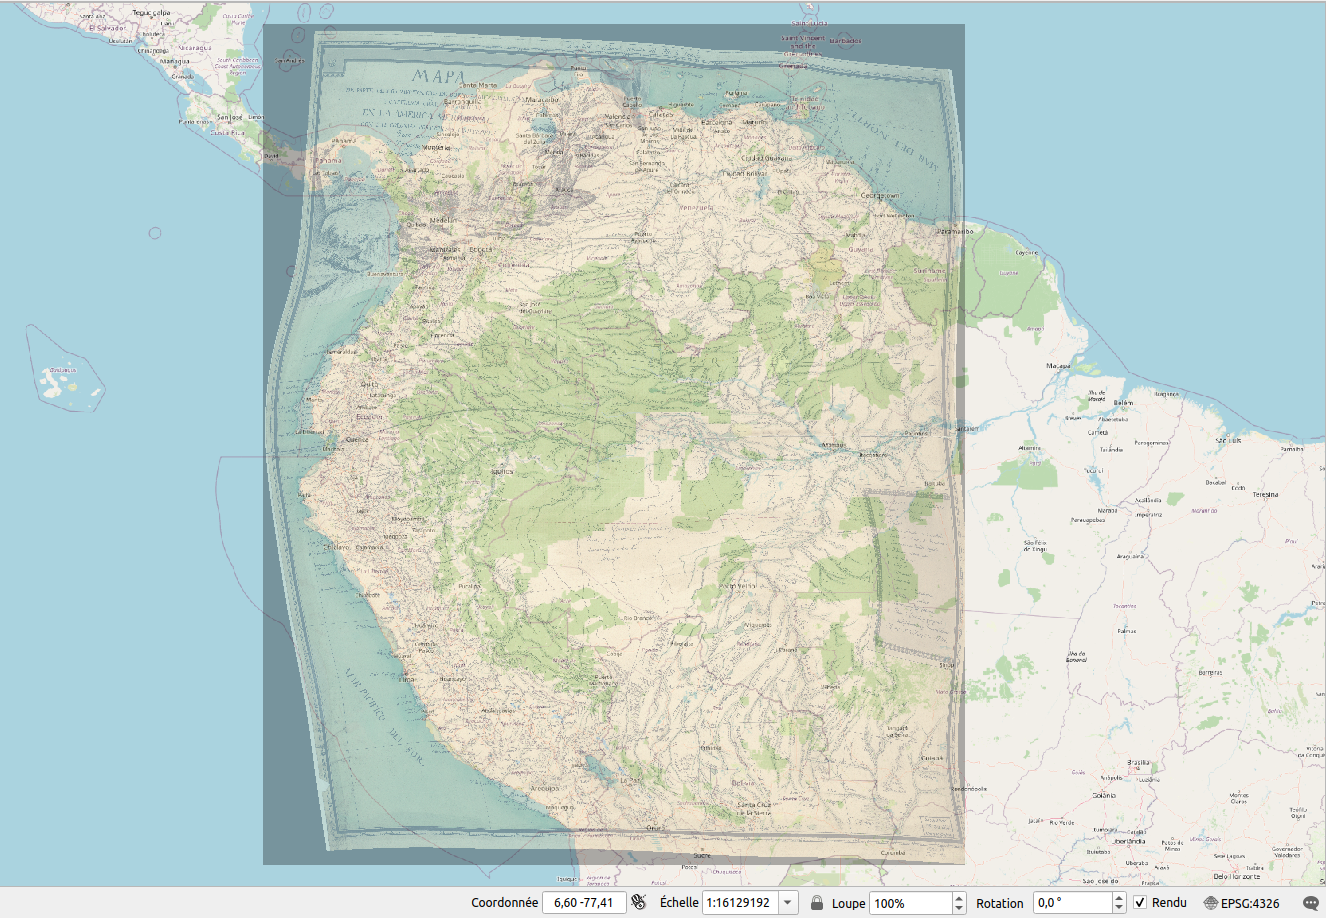
\includegraphics[width=18cm]{imgQgis.png}
    \caption{Géoréférencement de la Carte de Francisco Requena dans le logiciel Qgis.}
    \label{douzeFig}
\end{figure}

Nous avons fait un premier test pour essayer de comprendre comment fonctionne le système de géoréférencement sur un exemple de cartes que nous serons confrontés à utiliser au cours du projet, pour avoir une idée des difficultés et des enjeux du processus et pour savoir combien de temps ça prendrait de travailler avec des sources de ce type. Pour l’établissement d’une carte ancienne non géoréférencée, c’est un travail exhaustif qui doit être soucieux du détail, un travail à partir de la recherche des points de correspondances, nous avons dû beaucoup retravailler l’image de la carte ancienne, c’est un travail qui, pour être parfait, prend environ quatre heures pour une personne qui a de l’expérience.  

Pour établir la partie finale du projet qui est de rendre une base de données historiques et géographiques des Indes Occidentales à partir du Dictionnaire d’ Antonio de Alcedo, une fois la base de données complétée et enrichie avec des coordonnées géographiques, il sera possible de charger le fichier csv dans le logiciel de système d’informations géographiques Qgis, de cette façon il sera possible d’avoir les points de localisation pour commencer à manipuler les couches et rendre cependant plus lisibles les objectifs futurs du projet. 

Avoir pu essayer le logiciel QGIS et le géoréférencement des cartes anciennes, a rendu mon passage à ma plateforme géomatique dans le cadre de mon stage encore plus intéressant et avec encore plus de défis de vouloir représenter une cartographie moderne de l’Amérique Hispanique du XVIIIe siècle. Car définir les stratégies de ce qui sera présenté dans les cartes joue un rôle très important pour le rendu du projet, car représenter l’urbanisation de l’Amérique hispanique n’est pas seulement délimiter les territoires entre les empires portugais ou espagnol, c’est un enjeu tout autour de la compréhension d’une histoire coloniale d’une partie du XVIIIe siècle, ce projet pourra avoir plusieurs rendus possibles, soit historiques, géographiques, anthropologiques, statistiques, etc. 

Pour visualiser ce projet en tant que cartographie moderne, il pourra aider les étudiants, les chercheurs et la population à comprendre une évolution urbanistique selon l’histoire, à travers des projets en humanités numériques qui ont pour objectif de valoriser cette histoire, conserver et diffuser en open accès. 
	
	\chapter*{Conclusion}
	\addcontentsline{toc}{chapter}{Conclusion}

Au départ, concernant le projet \textit{ANR TopUrbi}, j’ai vu mon travail dans le cadre de stage comme une opportunité pour le projet et au sein de la plateforme géomatique de l’\Gls{EHESS} d’initier la partie en humanités numériques pour l’analyse et le traitement de la donnée. C’était également une réelle opportunité pour moi d’être présente au début du projet, de pouvoir participer à cette étape initiale de prise en main des décisions pour établir une stratégie numérique pour le traitement ciblé du Dictionnaire d’Antonio de Alcedo. 

Pendant ces cinq mois de stage, nous avons pu nous rendre compte de la richesse historique et géographique des informations du Dictionnaire, mais aussi de la complexité de comprendre une source de l’Amérique Coloniale du XVIIIe siècle. C’est à ce moment que nous avons entrevu l’importance d’un travail interdisciplinaire, dans lequel il y a beaucoup d’échanges et de partages entre les humanités numériques et les sciences sociales. Au sein de ce projet, nous avons eu l’opportunité d’être en contact dans un premier temps avec des historiens spécialisés dans l’Amérique Hispanique, des documentalistes, des anthropologues pour pouvoir enrichir notre manière de comprendre le sujet et notre source. 

Au cours de notre travail nous avons tenté également d’élaborer plusieurs outils qui correspondaient à nos exigences. Nous devions d’abord comprendre la source à laquelle nous étions confrontés pour travailler à notre projet, comprendre la manière de fonctionnement des documents qui nous ont été fournis par le projet similaire et en collaboration avec le nôtre, le projet HGIS de las Indias, afin d’aboutir à l’élaboration d’un processus qui allait nous faire à parvenir à notre but de constituer une base de données historiques et géographiques de l’Amérique Hispanique à partir du Dictionnaire historique et géographique d'Antonio de Alcedo.

Le traitement automatique est un processus exhaustif qui nécessite beaucoup de  compréhension de la source. C’est une succession des procédures comme la récupération des images, faire l’OCR des images, corrections des erreurs d’OCR, établissement d’un fichier en XML TEI, rédaction d’un script en langage de programmation capable de lire et de récupérer les informations d’une source avec des métadonnées et à la fin nous rendre un fichier dans un format de base de données, capable de stocker de la donnée historique et géographique.

Au fur et à mesure de la période de stage nous avons procédé à plusieurs méthodes afin de travailler notre source avec la finalité d’en ressortir divers éléments et données. L’analyse et la  structuration du texte étaient une étape exhaustive et nécessaire pour mettre en place des scripts en langage de programmation en Python, cela nous a permis de mettre à notre disposition une démarche afin d’accomplir partiellement l’objectif de ce stage : une base de données historiques et géographiques du Dictionnaire d’Antonio de Alcedo. 

A partir de l’alignement de notre source et grâce aux outils numériques nous avons pu constituer notre base de données et dans un premier temps relier cette base de données avec les bases de données Hgis de las Indias et GeoNames ; cependant la base n’est pas complète avec des coordonnées géographiques et pour l’avenir du projet il sera nécessaire de travailler sur les toponymes pour la désambiguïsation des lieux. 

Nous avons dû retravailler le fichier en métadonnées du texte brut du dictionnaire pour qu’il soit lu comme un fichier en XML TEI, nous avons mis en place des scripts en Python, pour, à partir de ce fichier en métadonnées, constituer une base de données en format fichier csv, ensuite nous avons pu relier notre gazetier aux gazetiers HGIS de las Indias et GeoNames automatiquement et récupérer les coordonnées géographiques. 

En parallèle avec notre objectif initial du stage nous avons pensé, pour la désambiguïsation des lieux, à mettre en place une première procédure en Traitement automatique des langues avec le support d’un script en langage de programmation et du logiciel tagtog. Ces annotations dans les entrées du Dictionnaire nous ont permis de faire une analyse plus au moins lexique du texte, et de tester notre compréhension du sujet. 
	
Cela aidera le travail futur d’entamer une discussion plus approfondie sur les choix des étiquettes à annoter par la suite et au travail de désambiguïsation de lieu et confirmera si le travail de récupération des coordonnées géographiques des lieux qu’on cherchait était bon, car il est possible d’avoir deux lieux avec le même nom. De même, en pensant à l’avenir du projet, nous avons pu faire les premiers tests avec les sources complémentaires qui seront utilisées par la suite du projet, comme les cartes anciennes dans le logiciel de système de l’information géographique QGIS, pour que je puisse prendre en main le logiciel et également ressentir les enjeux de travailler avec ces sources dans cet outil. 

Nous avons pu réaliser notre travail dans le meilleur des cadres, avec le partage et en commun, et même si j’ai pu rencontrer des difficultés tout au long de cette période, c’était bien d’avoir commencé mon stage au même temps que la partie technique en humanités numériques, c’était également une difficulté, car il n’y avait presque rien de défini ; ainsi partir du début a pris énormément de temps pour analyser nos sources et mettre en place une stratégie de plan d’avancement. Nous avons dû faire plusieurs allers-retours, car du fait que c’était une innovation nous avons dû tester de plusieurs manières nos choix de modules pour le traitement automatique au travers d’un langage de programmation. J’ai pu rencontrer des difficultés pour développer les scripts, car c’était également la première fois pour moi d’établir cette démarche pour le traitement automatique. 

Cependant ce stage a été très important pour moi, en tant qu’étudiante et jeune sur le marché, pour mettre en place les connaissances acquises au sein de ma formation en humanités numériques, j’ai appris à travailler en équipe au sein d’une structure interdisciplinaire, à améliorer la communication, le partage des tâches, à prendre en compte les avis des plus expérimentés, à pouvoir toujours demander de l’aide quand c’était nécessaire, mener un projet, comprendre les difficultés, les enjeux, et à ne pas avoir peur d’essayer de nouveaux outils et d’effectuer de  nouvelles démarches. 
	


%imprimer séparément les deux listes


	%les annexes
	\appendix
    \addcontentsline{toc}{part}{Annexes}
	\chapter{Scripts en Python}
	
	Pendant toute la durée de stage, le travail dépend de la création et de l'éxecution de divers scripts utilisant le langage Python. Ces scripts ont été présenté et expliqué partiellement dans le mémoire. Il est possible de retrouver chacun de ces scripts sur le Github de la Platerfome Géomatique, ainsi que la façon dont ils peuvent être éxecutés: https://github.com/PSIG-EHESS/Stage\_ANR\_TopUrbi/tree/branche\_anahi
	
	
		\section{Corpus}
		\noindent \textbf{Dictionnaire1} : Figure 3.1 - Structure du Dictionnaire - Tome I.  \\
		\textbf{Dictionnaire2} : Figure 3.5 - Ajouts et corrections du Dictionnaire - Tome I.\\
		
		Images de la sctructure du Dictionnaire d'Antonio de Alcedo, Tome I.
	
		\section{Les fichiers en XML}
		\noindent \textbf{image2} : Figure 3.2 - Fichier initial avec des métadonnées - Tome I. \\
		\textbf{image3} : Figure 3.3 - Fichier initial avec des métadonnées: Le choix des balises - Tome I. \\
		
		Encodage partial du Dictionnaire d'Antonio de Alcedo.
		
	\section{TEI}
\noindent \textbf{TEI} : Figure 3.4 - Adaptations en TEI du fichier initial - Tome I. \\
	
	Adaptations en TEI du fichier initial pour l'application du script en python.
	
	\section{GeoNames}
\noindent \textbf{image04} : Figure 3.6 - Résultat de la Recherche des lieux\\
	
	Script en Python permettant de relier les deux bases de données, le Dictionnaire d'Alcedo et la base de données GeoNames.
	
	\section{Annotations}
\noindent \textbf{image5} : Figure 4.1 - Annotation des entités nommées - Tome V, id = 16020.\\
	\textbf{img1} : Figure 4.2 - Annotation des entités nommées - Tome V, id = 15487.\\
	\textbf{imag06} : Figure 4.3 - Annotation des entités nommées - Tome V, id = 17774.\\
	\textbf{image07} : Figure 4.4 - Annotation des entités nommées - Tome V, id = 17750.\\
	
	Application des entités nommées sur l'application tagtog.
	
	\section{Cartographie}
\noindent \textbf{Requena carte} : Figure 4.5 - Carte de Francisco Requena(1796)\\
	\textbf{imgQgis} : Figure 4.6 - Logiciel Qgis \\
	
	Utilisation de la carte ancienne  de Francisco Requena (1796) pour le géoreferencement dans le lociel QGIS.
	
	\chapter{Glossaire}
	
	Le glossaire contient les définitions des mots clés en ordre aphalbéthique de notre projet.\\

	
	\noindent \textbf{API}: Interface de programmation d'application est un protocole qui permmet à un programme de communiquer avec un autre programme.\\
	
	\noindent \textbf{FAIR} Findable, Acessible, Interoperable, Reusable, sont des préconisations simples pour le partage de données. \\
	
	\noindent \textbf{Géomatique}: Ensemble d'outils et méthodes permettant d'acquérir, de répresenter, d'analyser et d'intégrer des données géographiques. \\
	
	\noindent \textbf{Reconnaissance Optique des Caractères}: Proceder permettant de transformer les images d'un texte en des fichiers électroniques au format texte.\\
	
	\noindent \textbf{Regex} Expression régulière est une chaîne de caractère, écrite selon une syntaxe precise qui permet de détecter des motifs dans du texte.\\
	
	\noindent \textbf{Système d’Information Géographique} Un système d’Information Géographique(SIG) est un outil informatique permettant de représenter et d’analyser toutes les choses qui existent sur terre ainsi que tous les événements qui s’y produisent. \\
	
	\noindent \textbf{Traitement automatique des langues}: Est un domaine de recherche pluridisciplinaire à l’intersection de la linguistique et de l’informatique – et désormais de l’intelligence artificielle, ou plus précisément de l’apprentissage artificiel. \\
	
	\noindent \textbf{TEI}: La Text Encoding Initiative (TEI) est un consortium qui développe et maintient collectivement une norme pour la représentation des textes sous forme numérique. \\
	
	\noindent \textbf{XML}: XML signifie eXtensible Markup Language est une métalangage de balisage informatique, conçu pour stocker et transporter des données et pour être à la fois lisible par l'homme et par la machine.
	
	\chapter{Outils et programmes}
	
	Au cours de le stage nous avons pû utiliser de nombreaux logiciels, outils, modules et programmes. 
	
	\section{Géneral}
	
	\noindent \textbf{CSV} : https://docs.python.org/3/library/csv.html \\
	
	Le module csv implémente des classes pour lire et écrire des données tabulaires au format CSV. \\
	
	\noindent \textbf{LXML} : https://lxml.de \\
	
	Module Python permettant de manipuler des données xml. \\
	
	\noindent \textbf{GEOCODER} : https://geocoder.readthedocs.io/ \\
	
	Geocoder est une bibliothèque de géocodage simple et cohérente écrite en Python. Traiter avec plusieurs fournisseurs de géocodage différents, tels que GeoNames, Google et etc.
	
	\noindent \textbf{GLOB} : https://docs.python.org/3/library/glob.html \\
	
	Le module glob recherche tous les chemins correspondant à un motif particulier selon les règles utilisées par le shell Unix, les résultats sont renvoyés dans un ordre arbitraire. \\
	
	\noindent \textbf{PANDAS} : https://pandas.pydata.org/docs/ \\
	
	Pandas est une bibliothèque écrite pour le langage de programmation Python permettant la manipulation et l'analyse des données. \\
	
	\noindent \textbf{PYTHON} : https://docs.python.org/3/tutorial/index.html \\
	
	Python est une lagage de programmation qui permet une approche simple et efficace de la programmation orientée objet. Ce langage s'est propulsé en tête de la gestion d'infrastructure, d'analyse de données ou dans le domaine du développement de logiciels. \\
	
	\noindent \textbf{RE} : https://docs.python.org/3/library/re.html \\
	
	Ce document constitue un guide d'introduction à l'utilisation des expressions régulières en Python avec le module re. Il fournit une introduction plus abordable que la section correspondante dans le guide de référence de la bibliothèque.
	
	\section{Traitement automatique des langues}
	
	\noindent \textbf{TAGTOG} : https://www.tagtog.com/ \\
	
	Tagtog est un outil d’annotation du texte permettant d’annoter et de normaliser les entités nommées. Il est par exemple possible d’ajouter des étiquettes d’entités, des relations, et même de faire plusieurs niveaux d’annotations.
	
	

	\section{Visualisation des données} : 
	
	\noindent \textbf{DATAIKU} : https://www.dataiku.com/ \\
	
	Dataiku est une plateforme de Data Science collaborative, et qui permet le traitement analytique des données.
	
	\section{Coordonnées géographiques} : 
	
	\noindent \textbf{GEONAMES} : https://www.geonames.org/ \\
	
	GeoNames est une base de données géographiques GeoNames couvre tous les pays et contient plus de onze millions de noms de lieux téléchargeables gratuitement. \\
	
	\noindent \textbf{HGIS DE LAS INDIAS} : https://www.hgis-indias.net/ \\
	
	HGIS de las Indias est un projet et une base de données géographiques de l'Amérique Hispanique au XVIIe siècle. \\
	
	\noindent \textbf{QGIS} : https://www.qgis.org/fr/site/ \\
	
	QGIS est un logiciel SIG (système d'information géographique) libre multiplate-forme publié sous licence GPL. 
	
\printglossary[type=\acronymtype]

    \backmatter
    \printbibliography
	
    \listoffigures	


% index à mettre ici si index	
%	\printindex

%glossaire si glossaire
%	\printglossaries

% si figures
%	\listoffigures

%si tables
%	\listoftables

	\tableofcontents
	
\end{document}